\documentclass[12pt,a4paper,twoside,titlepage,openright]{book}
\usepackage[MeX]{polski}
\usepackage[utf8]{inputenc}
\usepackage{enumitem} % słownik pojęć
\usepackage{amsmath}
\usepackage{tabularx} % tabele
\usepackage[usenames,dvipsnames,svgnames,table]{xcolor} % kolory jak~się chce gdzieś użyć
\usepackage{graphicx} % żeby ryciny i~zdjęcia były
\usepackage{listings} % syntax highlighting
\usepackage{verbatimbox} % marginesy dla~tabel
\usepackage{emptypage} % usuwa nagłówki i~numery stron z~pustych stron
\usepackage{afterpage} % to zapobiega ustawianiu obrazka PO tym
\usepackage{filecontents} % pozwala na wstawienie bibliografi
\usepackage{setspace} % interlinia
\onehalfspacing
\graphicspath{{figures/}} %Setting the graphicspath
% PAGE LAYOUT
%\usepackage{showframe} % debug
\marginparwidth 0pt
\marginparsep 0pt
\usepackage[top=2.5cm,bottom=3cm,inner=4.5cm,outer=3cm]{geometry}

% HEADER, FOOTER
\usepackage{fancyhdr} 
\pagestyle{fancy}

%kropki w~spisie tresci
\makeatletter
\def\numberline#1{\hb@xt@\@tempdima{#1.\hfil}}
\makeatother

% CHAPTER TITLE

%kropki po~tytułach rodziałów
\makeatletter
\def\@makechapterhead#1{%
  \vspace*{50\p@}%
  {\parindent \z@ \raggedright \normalfont
	\ifnum \c@secnumdepth >\m@ne
	  \if@mainmatter
	   \huge\bfseries \@chapapp\space \thechapter.
	   \par\nobreak
	   \vskip 20\p@
	\fi
   \fi
   \interlinepenalty\@M
   \Huge \bfseries #1\par\nobreak
   \vskip 40\p@
  }}
\makeatother

% SPIS TREŚCI

%kropki w~spisie tresci
\makeatletter
\def\numberline#1{\hb@xt@\@tempdima{#1.\hfil}}
\makeatother

% TYTUŁY ROZDZIAŁÓW

%kropki po~tytułach rozdziałów
\makeatletter
\renewcommand*\@seccntformat[1]%
{\csname the#1\endcsname.\enspace}
\makeatother


% KONFIGURACJA WYGLĄDU NAGŁÓWKA TEGO CO SIĘ POWTARZA

\fancyhead{} 
\fancyhead[LE]{\rightmark}
\fancyhead[RO]{\leftmark}

% WYGLĄD TABEL

% vertical padding
\renewcommand{\arraystretch}{1.5}

% CODE LISTINGS 

\definecolor{mygreen}{rgb}{0,0.6,0}
\definecolor{mygray}{rgb}{0.5,0.5,0.5}
\definecolor{mymauve}{rgb}{0.58,0,0.82}

\lstset{ %
%frame=lines,
aboveskip=1.5em,
    belowcaptionskip=1.5em,
    xleftmargin=0.5cm,
  backgroundcolor=\color{white},   % choose the background color
  %basicstyle=\footnotesize,        % size of fonts used for the code
  breaklines=true,                 % automatic line breaking only at whitespace
  captionpos=b,                    % sets the caption-position to bottom
  commentstyle=\color{mygreen},    % comment style
  escapeinside={\%*}{*)},          % if you want to add LaTeX within your code
  keywordstyle=\color{blue},       % keyword style
  stringstyle=\color{mymauve},     % string literal style
}

\definecolor{maroon}{rgb}{0.5,0,0}
\definecolor{darkgreen}{rgb}{0,0.5,0}

\lstdefinelanguage{XML}
{
  basicstyle=\ttfamily,
  morestring=[s]{"}{"},
  morecomment=[s]{?}{?},
  morecomment=[s]{!--}{--},
  commentstyle=\color{darkgreen},
  moredelim=[s][\color{black}]{>}{<},
  moredelim=[s][\color{red}]{\ }{=},
  stringstyle=\color{blue},
  identifierstyle=\color{maroon},
  morekeywords={Page.DataContext,viewModel:NameViewModel}
}

%\setmonofont{Consolas} %to be used with XeLaTeX or LuaLaTeX
\definecolor{bluekeywords}{rgb}{0,0,1}
\definecolor{greencomments}{rgb}{0,0.5,0}
\definecolor{redstrings}{rgb}{0.64,0.08,0.08}
\definecolor{xmlcomments}{rgb}{0.5,0.5,0.5}
\definecolor{types}{rgb}{0.17,0.57,0.68}

%Poprawne wyświetlanie listingów c#
\lstset{language=[Sharp]C,
%captionpos=b,
%numbers=left, %Nummerierung
%numberstyle=\tiny, % kleine Zeilennummern
%frame=lines, % Oberhalb und unterhalb des Listings ist eine Linie
showspaces=false,
showtabs=false,
breaklines=true,
showstringspaces=false,
breakatwhitespace=true,
escapeinside={(*@}{@*)},
commentstyle=\color{greencomments},
morekeywords={partial, var, value, get, set},
keywordstyle=\color{bluekeywords},
stringstyle=\color{redstrings},
basicstyle=\ttfamily\small,
}

\begin{document}

% ################################
%        STRONA TYTUŁOWA
% ################################

\begin{titlepage}

%\newgeometry{inner=3cm,outer=3cm}

\vspace*{1cm}
\begin{center}
\begin{Large}
Uniwersytet Mikołaja Kopernika\\[1mm]
Wydział Matematyki i~Informatyki\\[1mm]
\end{Large}
\end{center}

\vfill

\begin{center}
{\Large Paweł Marcin Chojnacki}\\
nr albumu: 260082\\
informatyka
\end{center}

\vfill

\begin{center}
{\Large Praca magisterska}
\end{center}

\vspace{0.5cm}

\begin{center}
{\Huge \textbf{Porównanie wydajności współczesnych architektur sieci neuronowych}}
\end{center}

\vspace{2cm}
\hfill
\begin{minipage}{6.5cm}
Opiekun pracy dyplomowej\\
dr hab. Piotr Wiśniewski
\end{minipage}

\vfill

\begin{center}
Toruń 2018
\end{center}

\end{titlepage}

% odwracamy kartkę ze~stroną tytułową to nic nie~ma z~drugiej strony -> pusta strona
\clearpage{\pagestyle{empty}\cleardoublepage}

\tableofcontents

% ################################
%        SŁOWNIK POJĘĆ
% ################################

\chapter*{Słownik pojęć}
\markboth{}{Słownik pojęć}
\addcontentsline{toc}{chapter}{Słownik pojęć}
\begin{description}[style=nextline]
	\item[Klasyfikacja binarna] Typ zadania klasyfikacji, którego wyjście stanowi jedna z dwóch wzajemnie wykluczających się klas. Prostym przykładem jest system rozpoznający wiadomości email podzielone na dwie klasy "spam" oraz "nie spam".
%	Klasyfikacja binarna polega na jak najdokładniejszym stwierdzeniu posiadania cechy lub przynależności do kategorii danego obiektu.
%Najczęściej używane metody do klasyfikacji binarnej to: drzewa decyzyjne 
%Dane wejściowe należy przedstawić w formie macierzy. Każdy przykład do treningu i później klasyfikacji, musi być tych samych wymiarów. Wyjściem algorytmu klasyfikacji binarnej jest wektor z prawdopodobieństwem klasyfikacji każdego z przykładów. Wizualizacja funkcji, klasyfikującej czerwone i zielone kółka.
	\item[Regresja logistyczna] Metoda statystyczna używana do analizy zbioru danych, w którym istnieje więcej niż jedna zmienna determinująca wyjście. Wyjście jest prawdopodobieństwem na ile obiekt wejściowy przypomina każdą z klas modelu. Regresja logistyczna jest zazwyczaj używana do klasyfikacji binarnej. %Algorytm regresji logistycznej przyjmuje na wejściu dane: n-wymiarowy wektor liczb rzeczywistych [np. Obraz], zestaw wag o tych samych wymiarach, liczba rzeczywista, bias.
%Do wygenerowania wyjścia, wystarczy obliczyć y = wT (wagi transponowane) * x (wejście) + b (bias). Należy jeszcze zastosować operację, która pozwoli na ustawienie parametrów w przedziale 0-1. Całe powyższe równanie użyć jako wejście do funkcji sigmoidy. Sigm(z) = 1 / 1 + e-z. Jeśli z jest duże, sigmoida będzie bliska 1, jeśli z jest liczbą ujemną, sigmoida zbliży się do 0.
	\item[Funkcja kosztu] Funkcja służąca trenowaniu modelu regresji logistycznej. Pozwala na określenie odległości wartości wyjściowej sieci od celu (prawidłowej odpowiedzi). Celem sieci neuronowej jest zminimalizowanie funkcji kosztu dla sygnałów wejściowych nie spotkanych wcześniej.% Mając zestawy treningowe, można wytrenować algorytm tak, aby podawał wartości prawdopodobieństwa jak najbliższe zestawu treningowego. Chcemy ustawić wagi i bias tak, aby te parametry dawały prawidłową odpowiedź dla każdego przykładu uczącego. Funkcja kosztu ma następujący wzór:
	\item[Metoda gradientu prostego (ang. gradient descent algorithm)] Algorytm pozwalający znaleźć minimum funkcji kosztu. Technika ta minimalizuje błąd w odniesieniu do parametrów modelu zadanych do trenowania przez wyliczenie optymalnych wartości wag oraz progów.% płaszczyzna funkcji dla wszystkich możliwych argumentów, algorytm przechodzi z losowo rozpoczętego miejsca w miejsce gdzie jest najgłębiej. Mając funkcję kosztu J(w,b) szukamy miejsca w którym błąd algorytmu jest jak najmniejszy.
	\item[Wykres obliczeniowy (ang. computation graph)] Dekompozycja wyrażenia (matematycznego) w pojedynczych atomowych krokach. Używany do szukania miejsc możliwego zoptymalizowania funkcji. Każdą operację wyrażenia przedstawia się jako osobny węzeł w grafie skierowanym. Wykresów obliczeniowych używa się podczas ręcznej analizy funkcji błędu oraz jako wizualizacji obliczeń w wielu bibliotekach głębokiego uczenia maszynowego.
	\item[Funkcja aktywacji] Jedna z funkcji (zazwyzaj sigmoidalna lub rektyfikowalna jednostka liniowa) która przyjmuje zsumowaną wartość wszystkich wejść z poprzedniej warstwy sieci neuronowej i propaguje wartość wynikową do następnej warstwy.
	\item[Konwolucja] Termin w kontekście uczenia maszynowego odwołuje się do operacji konwolucji lub warstwy konwolucyjnej. Konwolucja polega na stworzeniu macierzy będącej mieszanką macierzy wejściowej z filtrem konwolucyjnym dając zestaw wag mniejszy od orginalnego wejścia i tworząc mapę cech.
	\item[Łączenie (ang. pooling)] Technika polegająca na redukcji danych wejściowych z poprzedniej warstwy konwolucyjnej. W łączeniu zazwyczaj używa się maksymalną wartość lub średnią z obszaru puli, który z kolei jest macierzą kwadratową o zadanym rozmiarze (2x2, 3x3 lub 5x5). Aby zmniejszyć obraz należy ustalić rozmiar filtra oraz wielkość kroku. Następnie wykonuje się przejscie po całym obrazie z nałożonym filtrem. Każde przesunięcie po sygnałach z warstwy poprzedniej zwraca nową wartość dla warstwy łączącej. Pozwala to ograniczyć ilość parametrów i wyodrębnić konkretne cechy obiektu.
	\item[Wsteczna propagacja błędu] Najważniejszy algorytm dla znajdowania optymalnych wag w sieciach neuronowych. Przechodzi on w dwie strony sieci, pierw od warstwy wejściowej do wyjściowej wyliczane są wartości każdego neuronu. Nastepnie wykonywany jest powrót z ostatniej warstwy do pierwszej wyliczając pochodne cząstkowe błędu w stosunku do każdego parametru (wagi i progu).
	\item[Wyrzucanie połączeń (ang. dropout)] Sposób na redukcję przeuczenia modelu względem danych treningowych przez regularyzację danych. Dokładniej polega na deaktywacji losowych neuronów w trakcie uczenia, zapobiega to sytuacjom kiedy dane treningowe są rozpoznawane zbyt dobrze, a nowe sygnały nieznane wcześniej mają dużo niższą jakość rozpoznania.
	\item[Epoka] Pełne przejście przez zestaw danych treningowych, tak że każdy element został przekazany do sieci jeden raz.
	\item[Model] Reprezentacja obiektu utworzonego w wyniku uczenia sieci neuronowej. Z założenia model jest tym lepszy im dokładniej przewiduje klasę obiektu, którego wcześniej nie spotkał.
\end{description}
 
% ################################
%        WSTĘP
% ################################

\chapter*{Wstęp}
\markboth{}{Wstęp}
\addcontentsline{toc}{chapter}{Wstęp}
Celem niniejszej pracy magisterskiej jest przedstawienie nowoczesnych (czyli z ostatnich pięciu lat) architektur sieci neuronowych oraz przegląd najpopularniejszych bibliotek implementujących algorytmy uczenia maszynowego, a w szczególności zoptymalizowanych do pracy z uczeniem głębokim na wielu procesorach graficznych. 

Głębokie sieci neuronowe, czyli zawierające więcej niż jedną warstwę ukrytą, znane są już od wczesnych lat 60tych XX wieku. Algorytmy uczenia maszynowego były bardzo aktywnie rozwijane w latach 1950 - 1971, fundusze na badania w czasach zimnej wojny były w USA kilkukrotnie wyższe w udziale PKB. W czasie kryzysu z roku 1981, nadzieje wojska amerykańskiego na sztuczną inteligencję wygasły powodując epokę znaną jako drugą zimę SI (ang. second AI winter). Brak funduszy na badania znacząco zahamował rozwój systemów samouczących i do 2012 roku była to dziedzina zarezerwowana głównie dla doktorów matematyki i informatyki (głównie statystyków). 

Powrót na pierwsze strony gazet popularnonaukowych spowodował Geoffrey Hinton, wykorzystując swoje idee sprzed lat na bardzo wydajnym sprzęcie. Mowa o dwóch kartach graficznych GeForce GTX 580 3GB\cite{NIPS2012_4824}, które przez tydzień trenowały architekturę do rozpoznania obrazów pod zawody ImageNet Competition 2012. Wcześniej takie zawody wygrywało oprogramowanie łączące wiele algorytmów uczenia maszynowego, stąd nagły zwrot w kierunku jednolitego narzędzia dającego tym lepsze rezultaty im więcej danych do uczenia dostanie. Pierwszy raz można było zobaczyć głębokie sieci neuronowe mające trafność powyżej 80\%. Po publikacji dokumentu \"ImageNet Classification with Deep Convolutional Neural Networks\" nastąpił gwałtowny rozwój start-upów związanych z Deep Learningiem. Moc obliczeniowa kart graficznych i dedykowanych układów tanieje z każdym rokiem. 

Kluczowe dla rozwoju dziedziny są karty graficzne firmy NVidia. Firma chcąc być liderem w rewolucji SI, zmieniła swój wizerunek z dostawcy rozrywki dla graczy na lidera urządzeń i oprogramowania stanowiącego podstawę systemów uczących. Przez nagłą modę, wszystkie obecnie używane narzędzia mają nie więcej niż 5 lat. Dziedzina jest tak dynamiczna że zdarza się iż literatura w czasie publikacji papierowej staje się nieaktualna. Dlatego wykorzystana w tej pracy literatura to głównie publikacje elektroniczne z serwisu arXiv, będące zazwyczaj jeszcze bez recenzji naukowej. 

Intensywność obliczeń potrzebnych do stworzenia dobrego modelu wytwarza konieczność przedstawienia problemów osób praktykujących Deep Learning. W rozdziale poświęconym wydajności architektur przedstawiono sposoby na uniknięcie najczęściej popełnianych błędów oraz zbiór powszechnie przyjętych praktyk. Wydajność jest rozumiana zarówno jako czas obliczeń potrzebny do uczenia modelu rozpoznawania danego mu zagadnienia oraz dokładność z jaką już nauczony program potrafi rozpoznać niespotkane wcześniej dane. Oba te parametry są od siebie zależne, koszt poprawy jakości predykcji algorytmu o ostatnie 1-2\% może wynosić setki tysięcy złotych. Składa się na to energia elektryczna, farma serwerów wyposażonych w karty graficzne oraz tygodnie czekania na wynik. Zmiany zachodzące w rozwoju sprzętu i technik przenoszenia cech między modelami pozwolą na tworzenie aplikacji w czasie rzeczywistym już za kilka do kilkunastu lat.

Architektury posiadają wiele hiperparametrów, które wpływają na precyzję, po zmianie wartości dowolnego należy zacząć pracę algorytmu od początku. Dlatego dobór odpowiednio bliskich ideałowi wartości na start jest niezwykle cenny. Na rok 2017, żadna biblioteka nie posiada wbudowanych automatów do poszukiwania optymalnych hiperparametrów, dobieranie ich dzieje się na intuicję wyrobioną dziesiątkami prób. Istnieje kilka nowatorskich technik strojenia hiperparametrów, które ze względu na to że zostały odkryte przez mało znanych badaczy, nie zostały jeszcze rozpowszechnione w dużych ośrodkach badawczych, te techniki również są na tyle nowe, że nie ma wydawnictwa branżowego opisującego ich użycia dla praktyków. Techniki strojenia to algorytmy pozwalające efektywnie zmniejszyć błąd klasyfikatora o 10-20\%, co wiąże się z dużo wyższą wydajnością, przy znikomym nakładzie pracy. 

Do prezentacji działania bibliotek, architektur i algorytmów użyty został gotowy zbiór danych. Zestaw danych prezentacyjnych pochodzi z serwisu Kaggle. Jest to zbiór zdjęć z prześwietleń rentgenowskich podzielony na dwie kategorie: płuca zdrowe i płuca z zapaleniem płuc. Dane są anonimowe i zostały zweryfikowane przez Kaggle. Na końcu pracy z danymi znajduje się porównanie z osiągnięciami społeczności. Badanym obszarem są zagadnienia klasyfikacji obrazów, przy pomocy tworzenia map cech każdej z klas. Na przykładzie zbioru zdjęć, prezentowany jest sposób wykorzystania gotowych modeli i metody optymalizacji je pod wybraną domenę. Takie podejście pozwala uniknąć wysokich kosztów tworzenia własnych modeli (co kosztuje kilka do kilkunastu tygodni obliczeń na wielu kartach GPU). 

Głębokie sieci neuronowe również świetnie się sprawdzają przy zadaniach rozpoznawania mowy, przetwarzaniu języka naturalnego i systemach rekomendacji, zagadnienia zbyt obszerne by zostały opisane razem.

Praca jest podzielona na etapy tworzenia modelu od dołu struktury sieci neuronowych. Rozpoczyna się od przedstawienia pojedynczych elementów i struktury matematycznej sieci. Następnie opisany jest każdy element tworzący gotową architekturę.
Wszystkie przedstawione kody źródłowe zostały napisane w języku Python 3.6. Staje się on dominującym językiem w uczeniu maszynowym, kosztem języka R. Python składnią jest zbliżony do pseudokodu, dodatkowo wszystkie popularne biblioteki udostępniają nakładki API dla Pythona. Książki wykorzystane w tworzeniu tego tekstu, zawierają wyłącznie kod Pythonowy (z kilkoma nawiązaniami do języków R i C++).

% ################################
%        NEURONY
% ################################

\chapter{Neurony}
W niniejszym rozdziale została przedstawiona idea sztucznego neuronu McCullocha i Pittsa. Opracowany model biologicznego neuronu z 1943 roku jest tak uniwersalny że do dziś stanowi podstawę budowy sieci neuronowych. Przedstawiono tutaj również w jaki sposób znaleźć mapę cech, czy mówiąc prościej jak nauczyć neurony rozpoznawać wzorce. Na końcu rozdziału opisane są możliwości jakie daje łączenie sztucznych neuronów w sieć.

Pierwszy model sztucznego neuronu był wyobrażeniem biologicznej reprezentacji neuronu mózgowego z lat 40tych XX wieku. Była to bardziej próba implementacji idei niż odwzorowanie prawdziwego odpowiednika, który jest bardziej złożony i nie do końca znany jest sposób jego zachowania. Zdefiniowany przez noblistę Ramon y Cajal'a w 1906 roku neuron jest specjalistycznym nośnikiem wszelkich informacji, a także elementem przetwarzającym wszystkie doznania, emocje, a także sterownikiem całego ciała. Uproszczeniem które pozwoliło na sprawną implementację jest wyodrębnienie zasady przetwarzania informacji bioelektrycznej do kilku prostszych operacji. Takie uproszczenie składa się z wielu sygnałów wejściowych, wagi przypisanej każdemu z tych sygnałów oraz pojedynczej wartości wyjściowej. Jak wielkie jest to uproszczenie widać przy porównaniu rysunku prawdziwego neuronu (w uproszczeniu) oraz sztucznego neuronu. Taka budowa choć bardzo banalna, daje wiele możliwości. Podstawową zaletą jest prostota odwzorowania w urządzeniach elektronicznych. Przed nadejściem ery komputerów klasy PC, stosowano maszyny nazywane perceptronami, dlatego obecnie można używać nazwy sztuczny neuron i perceptron prosty zamiennie. 

\begin{figure}[h]
	\centering
			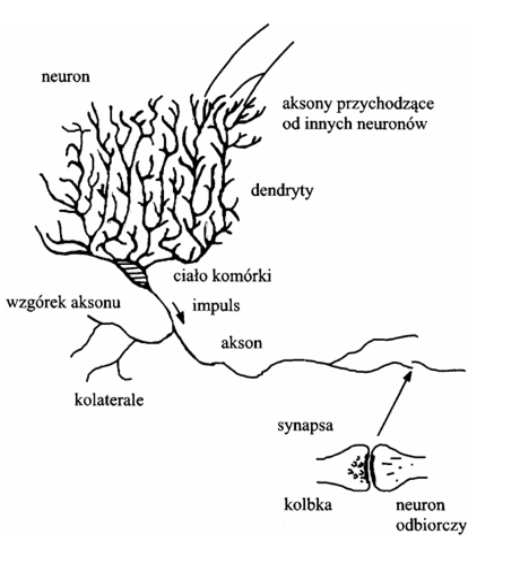
\includegraphics[resolution=100, scale=0.7]{neuronMozgowy.png}
		\caption{Wizualizacja uproszczonego modelu neuronu mózgowego.}
\end{figure}

\begin{figure}[h]
	\centering
			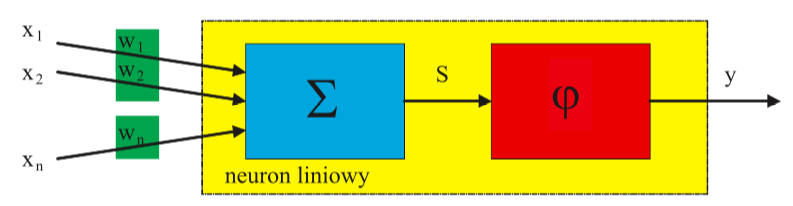
\includegraphics[resolution=100, scale=0.7]{sztucznyNeuron.png}
		\caption{Wizualizacja prostego sztucznego neuronu.}
\end{figure}

Model obliczeniowy został stworzony na podstawie algorytmu logiki progowej. 
Nazwa neuronu sztucznego została przyjęta w kręgach akademickich i biznesowych, stąd często osoby nie znające budowy mózgu ani działania sieci neuronowych mylnie nazywają zagadnienie Sztuczną Inteligencją, uproszczając skomplikowane procesy biologiczne do wzmacniania lub osłabiania sygnałów przekazywanych przez synapsy. Sieci neuronowe naśladują tylko jeden rodzaj pamięci, pamięć deklaratywną i w odosobnieniu nie tworzy inteligencji.

\section{Model perceptronu prostego}
Podstawowym elementem z których buduje się sieci neuronowe są sztuczne neurony, nazywane również perceptronami. Mają one być w rzeczywistości bardzo uproszczonym odwzorowaniem komórek nerwowych występujących w mózgu. Takie uproszczenia pozwalają na łatwą implementację modelu matematycznego, który ma reprezentować nasz obiekt i być tani w replikacji. Nawet po takim uproszczeniu jest on w stanie skutecznie naśladować \"uczenie\".
Sztuczny neuron jest funkcją matematyczną f(x,w) -> y. Można go opisać za pomocą modelu złożonego z:
\begin{itemize}
\item określonej liczby wejść n E N,
\item wagi, skojarzonej z każdym z wejść wi E R, i=1..n,
\item wybranej funkcji aktywacji FI: R -> R
\end{itemize}

Charakterystycznym elementem budulca sieci jest wiele wejść i tylko jedno wyjście, dlatego tak łatwo stworzyć model będący funkcją matematyczną.
Dane wejściowe oraz wyjściowe mogą przyjmować wartości z ograniczonego przedziału. Wartości przekazywane na wejściu i wartość wyjściowa zazwyczaj przyjmują znormalizowane wartości z przedziału xE [-1, 1] dla każdego z wejść, oraz y E[-1,1] dla wyjścia. W uproszczeniu można przyjąć y = SUM (wi * xi). wi są nazywane wagami (dawniej wagami synaptycznymi) i podlegają zmianom w trakcie uczenia neuronu. Wagi stanowią zasadniczą cechę sieci neuronowych działających jako adapcyjne systemy przetwarzania informacji. Zsumowana wartość jest wejściem dla funkcji aktywacji neuronu. Funkcja aktywacji zwyczajowo ma kształt sygmoidy, ale stosowane są obecnie również funkcje nazywane rektyfikownymi jednostkami liniowymi. Funkcja progowa ma za zadanie symulację zachowania przekaźnika synapsy, po przekroczeniu określonego progu aktywuje się dane zachowanie lub jak na przykładzie obrazów rozpoznanie cechy.

Ta prosta jednostka stanowi dziś podstawę budowy każdej sieci neuronowej. Aby funkcja zwracała oczekiwane wyniki, wagi powinny być poprawnie ustawione. Początkowo wagi ustawiano ręcznie za pomocą operatora (osoby przełączającej fizyczne kable), który wcześniej przeliczał je dla odpowiednich parametrów wejścia\\wyjścia. W latach 50tych perceptron stał się pierwszym modelem umiejącym samodzielnie wyliczyć poprawnie wagi definiujące zadaną klasę na podstawie przykładów. Wagi w zależności od wartości mogą sygnał wejściowy wzmocnić gdy waga jest większa od 1, lub stłumić gdy waga jest mniejsza niż 1. To pozwala wyuczonemu już perceptronowi na porównanie cechy obiektu wejściowego z tym co potrafi rozpoznać. 

W jaki sposób sztuczny neuron jest w stanie rozpoznać sygnał wejściowy? Do wyjaśnienia zjawiska w literaturze zazwyczaj prezentuje się przedstawienie modelu w notacji wektorowej.
X = [x1,x2,...,xn] - wektor wyznaczający punkt w n-wymiarowej przestrzeni, nazywanej przestrzenią wejść oraz , W = [w1, w2, ..., wn] - wektor wyznaczający punkt w n-wymiarowej przestrzeni, nazywanej przestrzenią wag. W ten notacji można wyrazić wyjście neuronu jako y= W(Transponowane) X. Wartość wyjściowa neuronu y, będzie wyższa im bliższe będzie położenie wektorów.

\begin{figure}[h]
	\centering
			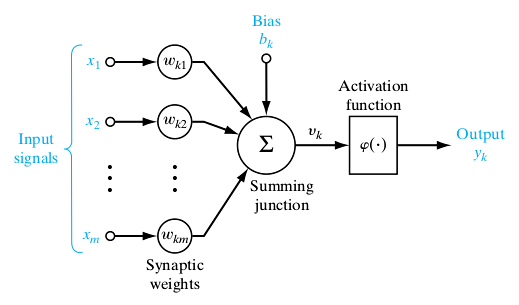
\includegraphics[resolution=100]{Neuron.png}
		\caption{Prosta reprezentacja neuronu.}
\end{figure}


\section{Co to jest sieć neuronowa?}
Koncepcja sztucznej sieci neuronowej to połączenie wielu neuronów w jeden obiekt. Pozwala to na rozpoznawanie bardziej skomplikowanych wzorców i większej różnorodności typów obiektów niż klasyfikacja binarna. Zwykła sieć neuronowa składa się z trzech warstw węzłów. Warstwa pierwsza stanowi warstwę wejściową sieci i składa się z sygnału wejściowego.

Kolejna warstwa jest nazywana warstwą ukrytą, użytkownik nie ma dostępu do niej, przypomina czarną skrzynkę. Nie można zaobserwować co się wewnątrz niej dzieje, użytkownik widzi jakie są dane wejściowe, wartości które powinny zostać zwrócone (w ostatniej warstwie), ale nie ma informacji co jest i powinno się znajdować w tej warstwie podczas trenowania sieci.
Ostatnia warstwa, pojedynczy węzeł nazywany jest warstwą wyjściową. Pobiera wektor wartości wyjściowych z poprzedniej warstwy (ukrytej) i na nim zostaje obliczona wartość wyjściowa (odpowiedź).

Taka architektura nazywa się siecią dwuwarstwową. Dane wejściowe, mimo że tworzą pierwszą warstwę nie są liczone w nazewnictwie.
Z warstwami ukrytą i wyjściową powiązane są parametry w (ang. weight) oraz b (bias), oznaczające kolejno: macierz wag oraz wektor progów.

\begin{figure}[h]
	\centering
			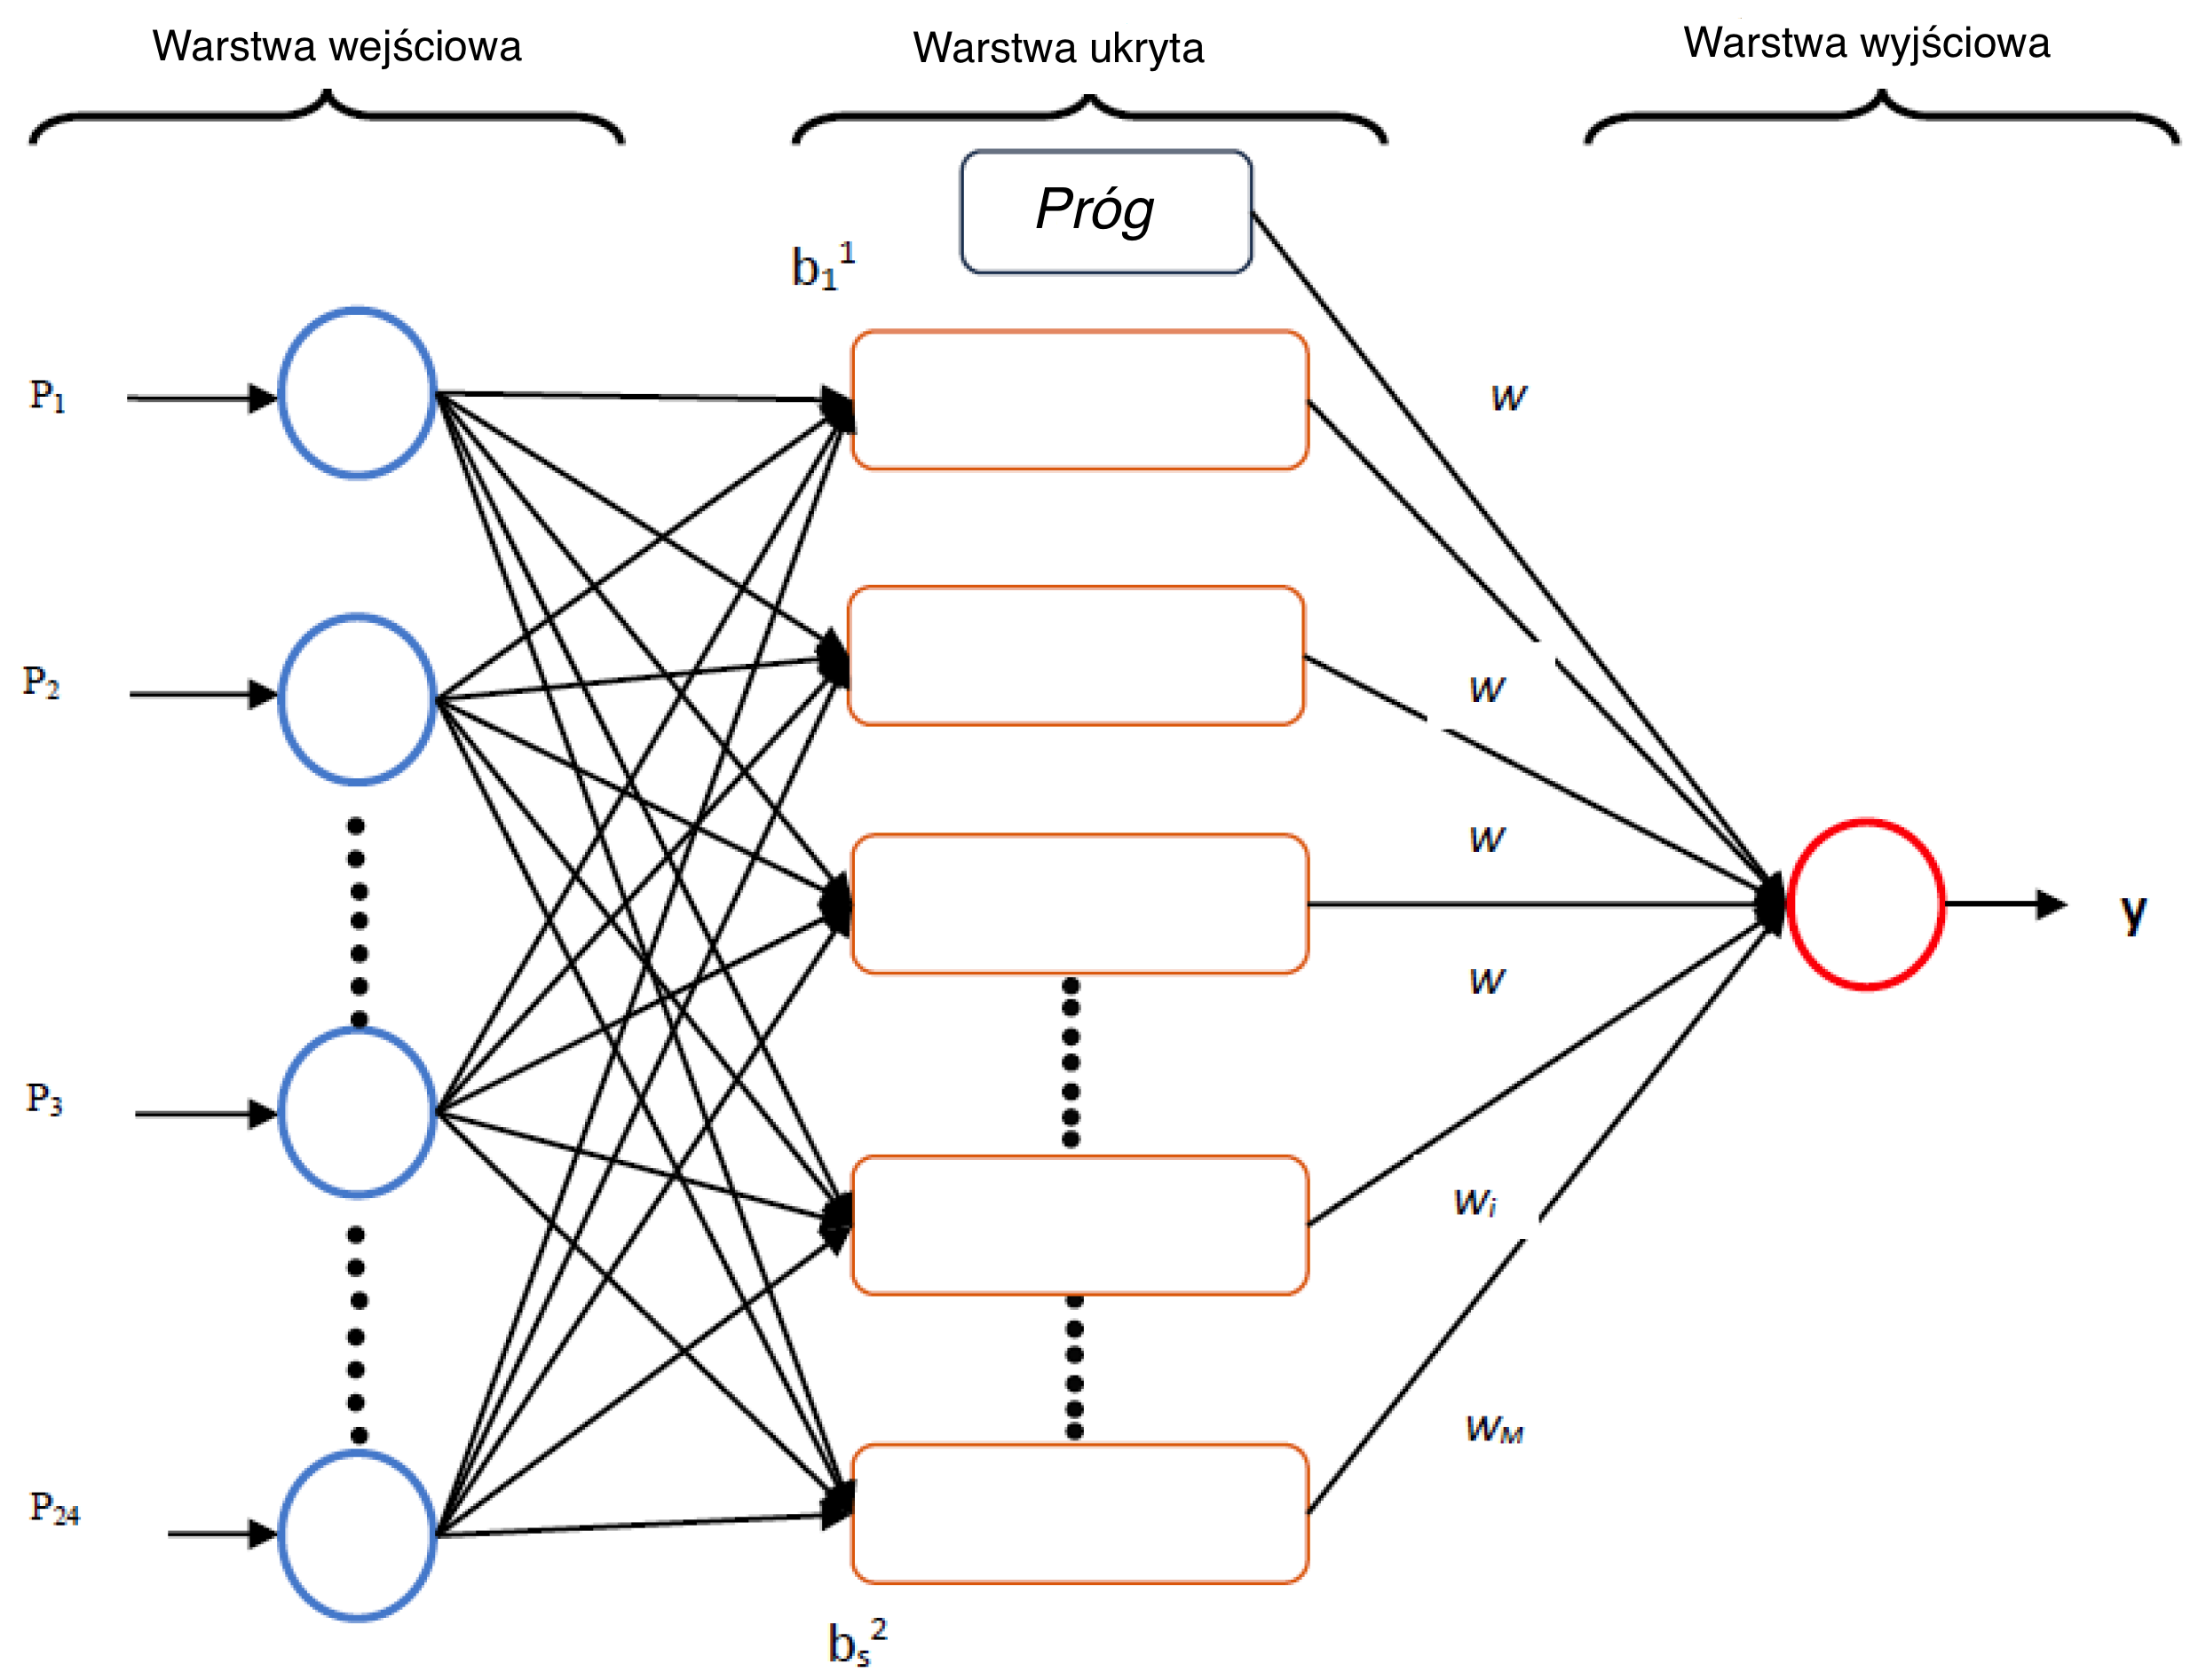
\includegraphics[resolution=100]{SiecNeuronowa.png}
		\caption{Prosta sieć neuronowa złożona z dwóch warstw.}
\end{figure}

\section{Jak uczyć sieci neuronowe}
W obecnym momencie istnieją dwie możliwości by sieć posiadła umiejętność poprawnej klasyfikacji. Można wyznaczyć dla algorytmu zbiór opisanych sygnałów wejściowych wraz z oczekiwanym sygnałem wyjściowym, ten typ tworzenia modelu sieci jest uczeniem nadzorowanym, co jest szczegółowo omawiane w tej pracy. Drugim podejściem jest podanie sygnałów wejściowych bez opisów i oczekiwanych wartości wyjściowych, to podejście nazywa się uczeniem nienadzorowanym.

\subsection*{Uczenie nadzorowane}
Jest to typ uczenia maszynowego, które zakłada obecność ludzkiego nauczyciela. Nauczyciel zobowiązany jest stworzyć odpowiednie dane uczące. Takie dane są parą danych, wejściowego obiektu uczącego oraz prawidłową odpowiedź wyjściową do tej danej. System na podstawie tych danych ma nauczyć się przewidywać poprawną odpowiedź dla nowych danych, ze znanej mu domeny.

Zadania uczenie nadzorowanego dzielą się na dwie kategorie, regresję i klasyfikację. 

W problemie regresji próbuje się przewidzieć wyniki, które są wartościami ciągłymi, czyli mając jakieś dane próbuje się je mapować na funkcję ciągłą. 

W problemie klasyfikacji algorytm ma za zadanie przewidzieć wyniki będące wartościami dyskretnymi, uściślając jest to znajdowanie klas obiektów, na podstawie danych wejściowych.

Uczenie nadzorowane ma wiele zastosowań, do głównych należą (wraz z używanym typem sieci):
\begin{itemize}
\item przewidywanie cen nieruchomości (zwykła sieć neuronowa),
\item reklamy internetowe (zwykła sieć neuronowa),
\item rozpoznawanie mowy (rekurencyjna sieć neuronowa),
\item tłumaczenie maszynowe w translatorach (rekurencyjna sieć neuronowa),
\item samochody autonomiczne (sieci hybrydowe lub inne niestandardowe sieci),
\item rozpoznawanie obiektów na obrazach (konwolucyjna sieć neuronowa).
\end{itemize}
Ostatnie z wyżej wymienionych zastosowań jest tematem badanym w tej pracy.

Uczenie nadzorowane dzieli się również binarnie ze względu na strukturę dostarczonych danych. Pierwszy rodzaj danych, dane zawierające konkretną strukturę, zazwyczaj tabela, są bardzo dobrze obsługiwane przez większość znanych wcześniej algorytmów uczenia maszynowego i nie wymagają ogromnej mocy obliczeniowej. Choć sieci neuronowe świetnie się sprawdzają przy tego typu danych, używanie ich ma sens dopiero gdy danych jest bardzo dużo (wielkość tabel przekraczające miliony rekordów). Drugi typ danych, nieustrukturyzowane zdjęcia, pliki audio, tekst, jest znacznie trudniejszy do rozpoznania przez komputer, za to dużo bardziej naturalny dla ludzi. Dzięki głębokim sieciom neuronowym i wielkiej mocy obliczeniowej komputerów, dokładność algorytmów uczących się na tego typu danych znacząco wzrosła, z 70\% do ok 95-99\% dokładności zależnie od ilości danych.

\subsection*{Uczenie nienadzorowane}
Uczenie maszynowe bez nadzoru nauczyciela jest drugim typem uczenia maszynowego polegającym na wyciąganiu wniosków z danych bez informacji zwrotnej o poprawności wniosków oraz bez określania etykiety danych. W algorytmach tego typu nie ma funkcji wyznaczającej poprawność utworzonego modelu. Najczęstszym zadaniem stawianym algorytmom uczenia nienadzorowanego jest wyznaczanie klastrów ze zbioru danych. W tej pracy temat uczenia bez nauczyciela nie jest poruszany.

\section{Elementy sieci neuronowych} 
Sieci neuronowe do poprawnego działania potrzebują więcej niż tylko połączenia ze sobą neuronów. Należy dobrać odpowiednie algorytmy korygujące błędy. Aby algorytm zatrzymał się w odpowiednim momencie z osobna trzeba zdefiniować warunki stopu dla epoki, ilość epok, rozmiar danych. Każda warstwa musi posiadać określoną funkcję aktywacji. Ostatnim opisanym elementem sieci są hiperparametry, czyli właściwości sterujące algorytmem by wiedział w jaki sposób wyznaczać pozostałe parametry.

\subsection{Metoda gradientu prostego}
Algorytm stosowany do szukania minimum lokalnego płaszczyzny wyznaczonej funkcją. Jest to bardzo prosta metoda optymalizacji stosowana do wyznaczania wag i progów. Płaszczyzna złożona z osi poziomych w i b oraz oś pionowa będąca wartością funkcji kosztu J(w,b). Algorytm mając początkowo losowe wagi i progi, rozpoczyna w tym losowym miejscu sprawdza wartość funkcji kosztu, następnie wykonuje małe przesunięcie w najbardziej stromym kierunku w dół płaszczyzny. Operacja zejścia powtarzana jest do zejścia do minimum lokalnego.

Schemat algorytmu:
Oznaczenia: 
Powtarzaj x razy {
	$w = w - \alpha * (dJ(w, b) / dw);
	 b = b - \alpha * (dJ(w, b) / db);$
}

\subsection{Funkcje aktywacji}
Budując sieć neuronową należy funkcje aktywacji dla warstw ukrytych oraz warstwy wyjściowej. Funkcje aktywacji są znane również jako charakterystyka neuronu. Charakterystyka neuronu jest elementem, który pośredniczy między zsumowanym pobudzeniem neuronu, a jego danymi wejściowymi. 

Najczęściej używaną charakterystyką była do niedawna funkcja sigmoidalna ponieważ ma wiele zalet:
\begin{itemize}
\item zapewnia łagodny gradient między wartościami 0 a 1,
\item ma gładką i prostą do liczenia pochodną,
\item jednym parametrem można dobrać kształt krzywej.
\end{itemize}
Definicja funkcji sigmoidalnej $ f(x) = 1 / (1+e^-z)$ .
Obecnie nie jest zalecane używanie funkcji sigmoidalnej poza przypadkami na warstwie wyjściowej w przypadku klasyfikacji binarnej, kiedy należy stwierdzić prawdopodobieństwo klasy obiektu. Dużo wydajniejszym odpowiednikiem jest następna funkcja.

Sprawną funkcją aktywacji jest tangens hiperboliczny. Jego wartości zawierają się między -1 i 1. Definicja funkcji tangensu hiperbolicznego $tanh(x) = (e^x - e^-x) / (e^x + e^-x)$. Jak widać na załączonych rycinach ta funkcja jest przesunięciem sigmoidy względem osi y, tak że przechodzi przez punkt (0,0). Dla warstw ukrytych charakterystyka neuronu będąca tangensem hiperbolicznym ma lepszą skuteczność. Mediana wartości wychodzących z warstw  ukrytych wynosi 0. Nie trzeba wtedy stosować skalowania względem sigmoidy, co znacząco ułatwia uczenie.

Zalecaną charakterystyką neuronu w dużych architekturach jest rektyfikowana jednostka liniowa. Definicja funkcji jest w porównaniu do pozostałych jest banalna $relu(z) = max(0,z)$. Jedynym problemem przy używaniu ReLU jest wyliczenie pochodnej kiedy argument z jest mniejszy od 0. W praktyce nie sprawia to większych problemów bo wartość zostanie ustawiona na 0, ale opracowano funkcję która jest pozbawiona tej niedogodności.

Nieszczelna liniowa jednostka rektyfikowana (ang. leaky Rectified Linear Unit) definiowana $f(x) = max(x, 0.01x)$. Pozwala to zmniejszyć efekt kiedy pochyła funkcji schodzi do 0, spowalniając uczenie. Niestety ta funkcja nie jest powszechnie używana w praktyce.

Należy podkreślić że w nowoczesnych sieciach neuronowych każda warstwa może posiadać indywidualnie ustanowioną funkcję aktywacji w zależności od architektury. Domyślnym wyborem funkcji aktywacji jest ReLU. 

\begin{figure}[h]
	\centering
			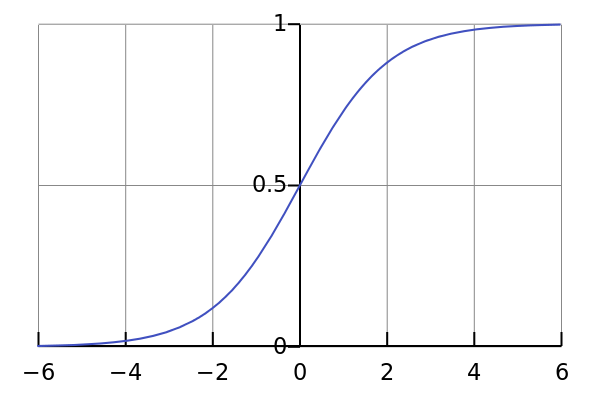
\includegraphics[resolution=100, scale=0.3]{Sigmoid.png}
		\caption{Wykres funkcji sigmoidalnej}
\end{figure}

\begin{figure}[h]
	\centering
			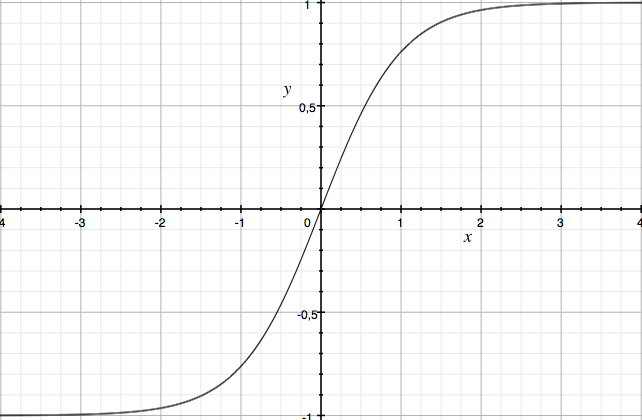
\includegraphics[resolution=100, scale=0.3]{Tangens.png}
		\caption{Wykres funkcji tangensu hiperbolicznego}
\end{figure}

\begin{figure}[h]
	\centering
			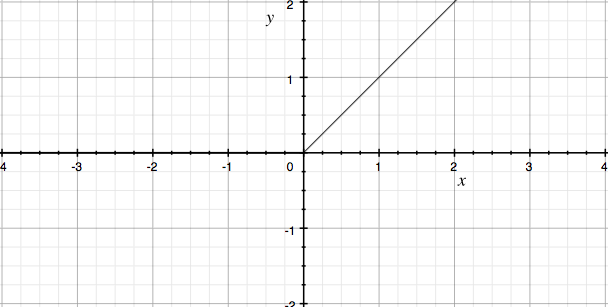
\includegraphics[resolution=100, scale=0.3]{ReLU.png}
		\caption{Wykres Rektyfikowanej jednostki liniowej}
\end{figure}

\begin{figure}[h]
	\centering
			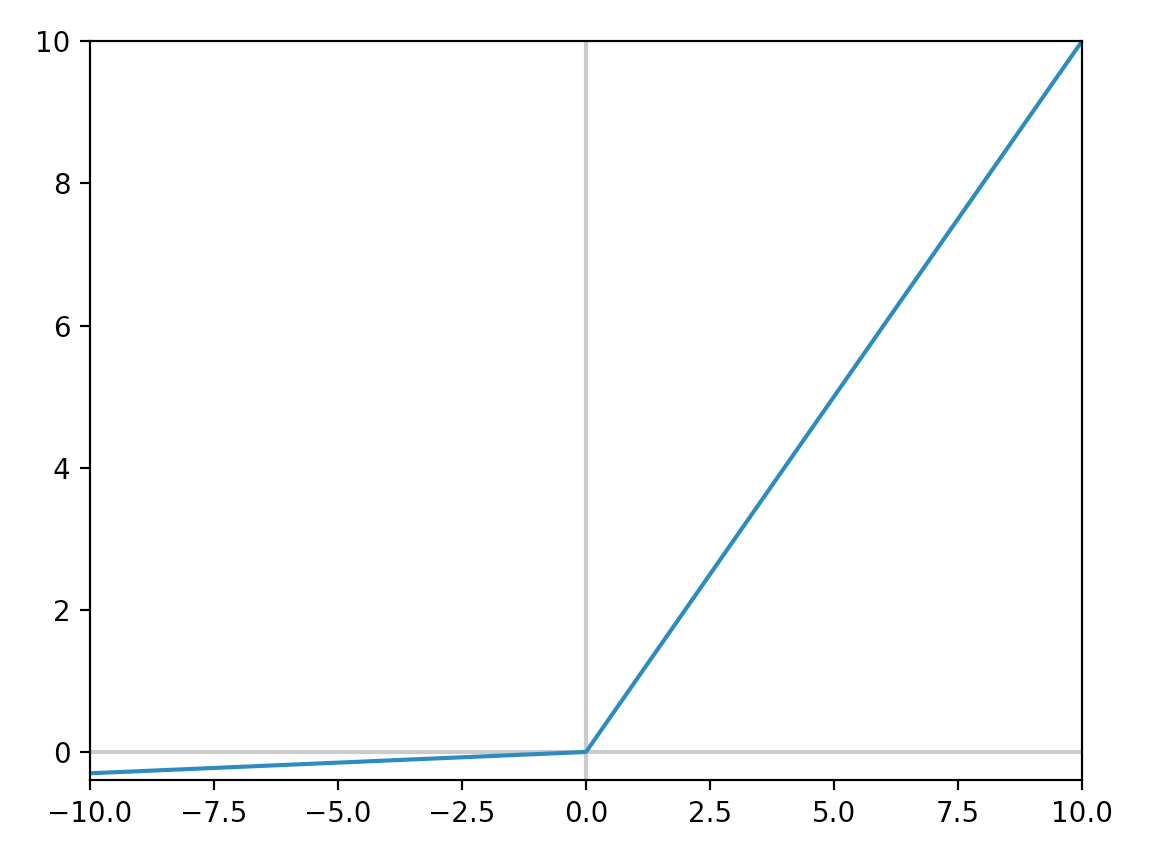
\includegraphics[resolution=100, scale=0.3]{leakyReLU.png}
		\caption{Wykres Nieszczelnej rektyfikowanej jednostki liniowej}
\end{figure}

\subsection{Parametry}
Najważniejszy element sieci neuronowej. Składa się na niego zbiór wag i progów (bias). Wagi wyznaczają sposób działania sieci, która ma nauczyć się dobrać odpowiednie parametry przy pomocy algorytmu uczącego, odpowiednio dobranych hiperparametrów oraz zbioru danych uczących. Wagi muszą być dobrane w sposób umożliwiający neuronom wykonanie czynności, których się od nich wymaga. Ze względu na ilość wag w głębokich sieciach, gdzie dla każdego z tysięcy neuronów może istnieć kilkaset wejść, proces musi być automatyczny. Sieć musi wiedzieć kiedy każdy z neuronów zwiększa swoją dokładność czy nie. Wagi i progi powinny być elastyczne i zmieniać się bardo szybko na początku procesu uczenia i tylko w niewielkim stopniu zmieniać wartości kiedy algorytm kończy proces uczenia.

\subsection{Hiperparametry}
Tworzenie dobrej sieci neuronowej wymaga nie tylko parametrów ale również dobrego doboru hiperparametrów. Elementy "ręcznie" dobierane dla algorytmu uczenia. Najczęściej ustawiane parametry dla sieci neuronowej to:
\begin{itemize}
\item stała uczenia,
\item ilość iteracji uczenia w jednej epoce,
\item ilość ukrytych warstw,
\item ilość ukrytych jednostek,
\item wybór funkcji aktywacji (ReLU, tangens, sigmoida),
\item parametry regularyzacji,
\item rozmiary próbek uczących,
\end{itemize}
i wiele innych mniej ważnych hiperparametrów

Są to parametry kontrolujące sposób wykonania algorytmu uczącego i w ostateczności to one mają największy wpływ na zwykłe parametry wagi i progi (bias). Nie został ustalony jednolity sposób doboru hiperparametrów. Zwyczajowo stosuje się metodę prób i błędów na podstawie tego jak algorytm się zachowuje.\cite{deeplearningAI} Za każdą zmianą wartości należy uruchomić algorytm i sprawdzić jak zachowuje się funkcja kosztu, jeśli maleje lepiej niż przy poprzednich wartościach można stroić dalej w tym kierunku. Dopieranie odpowiednich wartości niestety jest procesem empirycznym i należy wyrobić odpowiednią intuicję aby jak najtrafniej dobierać parametry od początku. Wartości te też nie są stałe, zmieniają się w zależności od dziedziny badanego zagadnienia. Być może najbliższe lata przyniosą dobry i spójny przewodnik dobierania najlepszych wartości, pozwoli to znacznie zautomatyzować proces.

\subsection{Wykres obliczeniowy}
Aby opisać organizację obliczeń podsekcję o wstecznej propagacji błędu, należy zformalizować operacje obliczeń. Robi się to za pomocą wykresu obliczeniowego. Węzły w grafie reprezentują skalary, wektory, macierze i tensory. Drugim elementem w grafie są operacje czyli proste funkcje z jedną lub większą ilością zmiennych. Graf obliczeniowy przydaje się kiedy istnieje zdefinowana funkcja bądź zmienna, którą należy zoptymalizować, w przypadku sieci neuronowych oczywistą jest funkcja kosztu.

Dla przykładu chcę obliczyć funkcję kosztu J o zmiennych a,b,c zdefiniowaną J(a,b,c) = 3(a+bc). Obliczenie tej funkcji składa się z trzech kroków, pierwszym jest policzenie b*c.
i = b * c
Następnym krokiem jest dodanie zmiennej a.
k = a + i
Trzecim i ostatnim krokiem jest wyjście funkcji kosztu J = 3k.
Graf obliczeniowy powyższej funkcji znajduje się na rysunku poniżej.

Do minimalizowania funkcji kosztu algorytm obliza pochodne w odwrotnej kolejności do przedstawionej na poprzednim przykładzie grafu.

\begin{figure}[h]
	\centering
			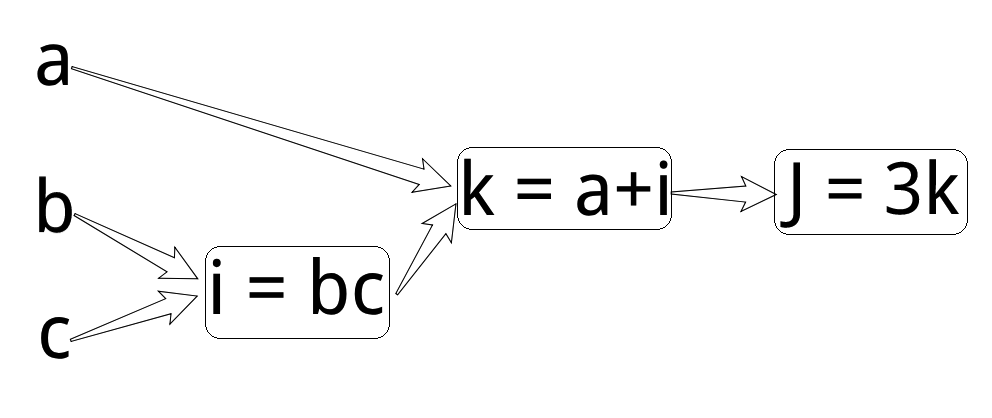
\includegraphics[resolution=100, scale=0.5]{ComputationGraph.png}
		\caption{Wykres obliczeniowy dla funkcji J(a,b,c) = 3(a+bc)}
\end{figure}

\subsection{Wsteczna propagacja błędu}
Algorytm wstecznej propagacji błędu został opracowany w latach 70tych, jednak używany dopiero ponad 10 lat później kiedy Rumelhart, Hinton i Williams wykazali skuteczność metody w strojeniu wag w ukrytych warstwach sieci.

Przekazując sygnał na wejście sieci zostaje on propagowany w przód przez wszystkie warsty do warstwy wyjściowej. Losowy neuron w warstwie ukrytej otrzymuje wartości wyjściowe z neuronów poprzedniej warstwy, mnoży każdy otrzymany sygnał z wagą przypisaną danemu wejściu i przekazuje zsumowany wynik do funkcji aktywacji. Każdy neuron wykonuje takie operacje do czasu trafienia na ostatnią warstwę gdzie sieć podaje juz oczekiwany wynik. Cały ten proces nazywa się propagacją w przód. Mając oczekiwany wynik na warstwie wyjściowej, zazwyczaj prawdopodobieństwo przynależności do każdej z uczonych klas należy wyliczyć funkcję błędu (ang. loss function). Funkcja ta pozwala określać odchylenie wyliczonego wyniku od właściwej odpowiedzi. Celem sieci jest zminimalizowanie błędu przez wyliczenie pochodnej z funkcji kosztu w stosunku do wag modelu.

Wsteczna propagacja błędu jest narzędziem używanym przez algorytm gradientu spadkowego aby wyliczyć gradient funkcji błędu. W trakcie przejścia wstecz przez sieć neuronową następuje korekcja wag. Przechodząc od wartości wyjściowej należy zmodyfikować wagi warstwy poprzedzającej tak by zmniejszyć wartość funkcji błędu.



Istnieją również analogiczne metod korekcji wag, jak szybka propagacja (ang. quick-propagation) oraz bardziej skomplikowane i ograniczone założeniami matematycznymi metoda gradientów sprzężonych i metoda Levenberga-Marquardta. Metody te są dużo szybsze od wstecznej propagacji błędu, ale przez swoje ograniczenia prawie nigdy nie są używane w praktyce. \cite{odkrywanieSieci}

%\subsection{Jak zbudować sieć neuronową}

% ################################
%        DEEP LEARNING
% ################################

\chapter{Deep Learning}
\section{Techniki tworzenia głębokich sieci}
W tym rozdział zostają przybliżone trzy interesujące techniki głębokiego uczenia. Zostały wybrane ze względu na ich obszerną ilość zastosowań oraz potencjał, który można wykorzystać przy rozpoznawaniu wzorców na obrazach. Następnie opiszę kilka bibliotek implementujących wsparcie dla większości architektur sieci przedstawionych w pracy. Biblioteki są wybrane na podstawie przekroju platform i języków mi znanych. 

\subsection{Sieci neuronowe}
Sztuczne sieci neuronowe zostały opisane w poprzednim rozdziale, tutaj uwaga skupia się na podziale na różne architektury, głębokości oraz rodzaj dodatkowych warstw, takich jak filtr cech.

\subsection{Convolutional Neural Networks}
Sieci konwolucyjne stosowane głównie do sygnałów wejściowych będących obrazem (zbiorem pikseli). 
\subsection{Recurrent Neural Networks}

\subsection{Fully Convolutional Networks}


% ################################
%        BIBLIOTEKI
% ################################
\chapter{Biblioteki implementujące uczenie głębokich sieci neuronowych}
Nagły wzrost zainteresowania sieciami neuronowymi, spowodował pojawienie się wielu bibliotek implementujących Deep Learning i przy okazji wiele pobocznych zadań Machine Learningu. Obecnie wiele z największych firm technologicznych próbuje wypromować własny stos technologiczny oparty o licencję Open Source. Otwartość nie wynika z dobroduszności i chęci dzielenia się ze społecznością, a  Wspólnym mianownikiem wszystkich narzędzi jest kompletne API dla użytkowników języka Python. Jest to język w którym najszybciej można znaleźć literaturę wprowadzającą w zagadnienie.

Na uwagę zasługuje fakt pojawienie się kilku bibliotek napisanych wyłącznie dla JavaScript'u. Ich zastosowanie jest nastawione na użytkowników gotowych modeli i ogranicza się głównie do importu zminiaturyzowanych wag na telefon by szybko odpowiadać na sygnały użytkownika takie jak zdjęcie z aparatu, bądź komendę głosową. 

\subsection{Tensorflow}
\begin{figure}[h]
	\centering
			
\includegraphics[resolution=100, scale=0.5]{Tensorflow.png}
		\caption{Logo biblioteki Tensorflow}
\end{figure}

Tensorflow jest pierwszą otwartoźródłową biblioteką dla obliczeń numerycznych uzywając grafów przepływu danych. Umożliwia praktykom uczenia maszynowego wykonywać intensywne obliczenia na danych przez wydajną implementację powszechnie używanych algorymtów głębokiego uczenia. Węzły w grafie przepływu są reprezentowane jako operacje matematyczne, zaś wierzchołki przedstawiają wielowymiarowe macierze (tensory) zapewniające komunikacje między wierchołkami i węzłami. Architektura tworzonych sieci w Tensorflow jest łatwa w modyfikacji, dlatego jeden model można wykorzystać do pracy z procesorami CPU, GPU, urządzeniami mobilnymi i chmurą mieszaną. \cite{DeepLearningTensorflow}

Pierwotnie Tensorflow umożliwiał pracę tylko z językiem Python. Od wersji 1.0 dodano eksperymentalne API do Javy i Golag. Ta wersja zadebiutowała z innowacyjnym narzędziem Tensorflow Debugger. Jest on narzędziem tekstowym do debugowania działających aplikacji.

Należy zaznaczyć że biblioteka jest wieloplatformowa i działa na wszystkich popularnych systemach operacyjnych:
\begin{itemize}
\item Windows
\item Linux
\item Mac
\item Android
\item iOS
\item Raspberry PI
\end{itemize}

Zestaw narzędzie zawiera Tensorflow Board graficzne oprogramowanie do analizy utworzonych modeli. Łatwość użycia i przyjęcie modelu Open Source sprawia że jest to najczęściej używana biblioteka podczas prac naukowych, o czym świadczy ilość cytowań[1]. Wiele firm wspiera projekt używając kodu i dodając do niego własne rozszerzenia, warto wymienić choćby kilku większych kontrybutorów:
\begin{itemize}
\item Google,
\item ARM,
\item Twitter,
\item Ebay,
\item Intel,
\item Qualcomm
\end{itemize}

Główne zalety:
\begin{itemize}
\item Największe zasoby dokumentacji i tutoriali,
\item Oglądanie w czasie rzeczywistym procesu uczenia przez Tensorboard,
\item Największa społeczność skupiona wokół projektu spośród wszystkich bibliotek,
\item Wspiera uczenie rozproszone na wielu maszynach,
\item Odmiany Tensorflow Lite i Tensorflow JS umożliwiają zastosowanie tych samych modeli na urządzeniach mobilnych i przeglądarkach
\end{itemize}

Tensorflow ma dwie wady, działające na niekorzyść osób zaczynających pracę z sieciami neuronowymi:
\begin{itemize}
\item Wymaga sporej ilości kodu do utworzenia działającego modelu, przez co uważany jest za bibliotekę niskopoziomową w porównaniu do pozostałych,
\item Kompletne wsparcie istnieje tylko dla języka Python, 
\item Jest dużo wolniejszy od CNTK i MXNet \cite{DBLP:journals/corr/ShiWXC16}
\end{itemize}

\noindent
\newline 
Dokumentacja: https://www.tensorflow.org/api\_docs/python/
\newline 
Kod źródłowy: https://github.com/tensorflow
\newline 
Licencja: Apache 2.0

\subsection{Keras}

\noindent
\begin{minipage}{\linewidth}
\begin{lstlisting}[caption=Skrypt najprostszego modelu sekwencyjnego (Keras w 30 sekund), label=lst:test]
from keras.models import Sequential
from keras.layers import Dense
model = Sequential()
model.add(Dense(units=64, activation='relu', input_dim=100))
model.add(Dense(units=10, activation='softmax'))
model.compile(loss='categorical_crossentropy',
              optimizer='sgd',
              metrics=['accuracy'])
model.compile(loss=keras.losses.categorical_crossentropy,
              optimizer=keras.optimizers.SGD(lr=0.01, momentum=0.9, nesterov=True))
model.fit(x_train, y_train, epochs=5, batch_size=32)
model.train_on_batch(x_batch, y_batch)
loss_and_metrics = model.evaluate(x_test, y_test, batch_size=128)
classes = model.predict(x_test, batch_size=128)
\end{lstlisting}
\end{minipage}

\begin{figure}[h]
	\centering
			
\includegraphics[resolution=100, scale=0.25]{Keras.png}
		\caption{Logo biblioteki Keras}
\end{figure}

Keras jest frameworkiem udostępniającym wysokopoziomowe API dla głębokich sieci neuronowych. Jego źródła zostały otwarte w 2015 roku. Społeczność skupiona wokół projektu wyróżnia się bardzo pozytywnym podejściem dla osób z poza środowiska naukowego i jest otwarta na propozycje rozwoju biblioteki. Nazwa Keras pochodzi od greckiego słowa κέρας oznaczającego róg, geneza nazwy wywodzi się z Odyseji. 

Założeniem François Chollet'a, czyli autora jest zwiększenie szybkości przeprowadzania ekperymentów, dlatego Keras ma wysokopoziomowe API udostępniające uruchomienie algorytmów głębokiego uczenia w kilku liniach kodu. Zalety wymieniane przez autora:
\begin{itemize}
\item Wspieranie łatwego i szybkiego prototypowania (przez modualrność, przyjazny interfejs, możliwośći rozszerzenia),
\item Wspiera konwolucyjne sieci neuronowe, rekurencyjne sieci neuronowe i umożliwia mieszanie obu,
\item Działa na CPU i GPU.
\end{itemize}

Działanie opiera się na wykorzystaniu rdzenia Tensorflow, CNTK lub Theano jako bibliotek wykonujących obliczenia. Potwierdza to idee stworzenia narzędzia dla szybkieko prototypowania modeli.

Do zalet można zaliczyć:
\begin{itemize}
\item Najszybsze prototypowanie ze wszystkich rozwiązań na rynku,
\item Uproszczony interfejs zachęca do eksperymentów osoby nie związane z Data Science,
\item Wbudowane wsparcie do pracy na GPU,
\item Wspiera strumieniowanie danych przez Spark,
\item Działa nie tylko na kartach NVidia, ale też Google TPU, AMD
\end{itemize}

Przy dłuższej pracy i bardziej skomplikowanych modelach wysokopoziomowość ogranicza elastyczność w działaniu. Nie ma tak wielu możliwości kontroli sieci jak pozostałe biblioteki, dlatego głównie poleca się ją dla nowicjuszy i eksperymentów przy standardowych typach sieci (konwolucyjnych, rekurencyjnych).

\noindent
\newline 
Dokumentacja: https://keras.io/
\newline 
Kod źródłowy: https://github.com/keras-team/keras
\newline 
Licencja: MIT

\subsection{PyTorch}
Oprogramowanie wywodzące się ze starej biblioteki Torch. Otwartoźródłowa paczka uczenia maszynowego dla języka Python. Główna biblioteka używana w Facebook'u do przetwarzania języka naturalnego. 

PyTorch dostarcza dwie wysokopoziomowe funkcjonalności:
\begin{itemize}
\item Obliczenia na tensorach z akceleracją obliczeń na GPU,
\item Głębokie sieci neuronowe zbudowane na automatycznie różniczkowalnym systemie taśmowym
\end{itemize}

Główne zalety:
\begin{itemize}
\item Proces modelowania jest prosty i przejrzysty dzięki architekturze opartej na programowaniu imperatywnym,
\item Dynamiczne generowanie grafu sieci,
\item Deklaratywna równoległość danych, czyli dzielenie sygnałów wejściowych na wiele mniejszych,
\item Najbardziej ''Pythoniczna'' składnia,
\item Zawiera sporą ilość pretrenowanych modeli i architektur, pozwalając na kombinację ich w nowe struktury,
\item Graf obliczeniowy jest generowany w trakcie działania programu, co pozwala na używanie dowolnego debuggera i nawet drukowanie obecnego stanu obliczeń na ekran, jest to spory potencjał na narzędzia interaktywne
\item Służy także jako alternatywa dla numpy z możliwością obliczeń na GPU,
\item Specjalnie napisane zarządzanie pamięcią GPU, pozwalające na niesamowicie wydajne zarządzanie pamięcią w porównaniu do konkurencji
\end{itemize}

PyTorch jest jednym z najmłodszych narzędzi, dlatego ma kilka poważnych wad:
\begin{itemize}
\item Nie jest zalecany do zastosowań produkcyjnych. Obecna wersja jest numerowana 0.4, wersja 1.0 była zapowiedziana na lato 2018. Na wrzesień 2018 brak informacji kiedy nastąpi premiera,
\item Brak gotowych narzędzi do monitoringu i wizualizacji procesu uczenia i podglądu grafu sieci
\end{itemize}

Język Pyro do programowania probalistycznego stworzony przez firmę Uber opiera się na PyTorch.

\begin{figure}[h]
	\centering
			
\includegraphics[resolution=100, scale=0.3]{PyTorch.png}
		\caption{Logo biblioteki PyTorch}
\end{figure}

\noindent
\newline
Dokumentacja: https://pytorch.org/docs/stable/index.html
\newline
Kod źródłowy: https://github.com/pytorch/pytorch
\newline
Licencja: Brak określonej. Prawa autorów zastrzeżone, oprogramowanie \"as is\".


\subsection{Tensorflow.js [Deeplearn.js]}
\begin{figure}[h]
	\centering
			
\includegraphics[resolution=100, scale=0.5]{TensorflowJS.png}
		\caption{Logo biblioteki Tensorflow.js}
\end{figure}

W 2017 roku został opublikowany projekt o nazwie Deeplearn.js z celem wprowadzenia uczenia maszynowego i głębokiego uczenia do przeglądarek internetowych bez konieczności korzystania z zewnętrznego API. 

JavaScript kojarzony jest przez starych programistów jako powolny interpretowany język ograniczony do pracy w obrębie jednego procesu procesora CPU. Aby uniknąć restrykcji wydajnościowych zaimplementowano wykonanie operacji na WebGL, przeglądarkowemu interfejsowi do OpenGL.

W maju 2018 zespół odpowiedzialny za rozwój DeepLearn.js został połączony z zespołem programistów pracujących przy Tensorflow, a biblioteka zmieniła nazwę na Tensorflow.js. Dostarcza calej mocy Tensorflow do przeglądarki czy dowolnego interpretera kodu Javascript jak Node.js.

Tensorflow.js nie ma wspólnej bazy kodu z Tensorflow, również filozofia działania jest inna. Należy podkreślić że zbieżność nazw wynika z połaczenia pracy dwóch zespołów w jedną jednostkę. Interfejs programistyczny udostępniany przez framework javascriptowy udostępnia zarówno niskopoziomowe elementy do uczenia maszynowego oraz wysokopoziomy interfejs wzorowany na tym z biblioteki Keras do tworzenia sieci neuronowych.

Biblioteka na podstawowym poziomie dostarcza dwa elementy:
\begin{itemize}
\item CoreAPI -- komponent zarządzający kodem niskopoziomowym,
\item LayerAPI -- komponent zbudowany na CoreAPI, udostępnia abstrakcje wyższego poziomu
\end{itemize}

Podstawową jednostką danych jest tensor, czyli zbiór wartości liczbowych ułożonych w tablicę jedno lub więcej wymiarową. Tensor definiuje się konstrukturem tf.tensor, gdzie należy określić tablice oraz kształt tensora. Istnieje wiele metod pozwalających na stworzenie tensorów róznych kształtów takich jak tf.zeros do wypełnienia podanego kształtu zerami, oraz takie jak tensor1d, tensor2d, tensor3d i tensor4d dla ułatwienia czytelności przy tworzeniu najczęściej używanych rozmiarów.
Tensory są niezmienne co oznacza że raz stworzony tensor nie może zmieniać wartości. 

Zmienne (ang. Variables) są inicjalizowane wartościami tensorów i można modyfikować ich wartości, używa się ich do trzymania i aktualizacji wartości w trakcie trenowania modelu.

Operacje (ang. Operations [Ops]) to metody pozwalające na modyfikacje danych. Tensorflow.js udostępnia całą gamę operacji do pracy z machine learningiem. Działają one na tensorach przez zwracanie wyniku operacji jako nowy tensor.

Powyższe struktury danych należą do CoreAPI, druga warstwa operacji LayerAPI operuje na wyższym poziomie abstrakcji i zapewnia zupełnie inne bloki do budowy sieci neuronowych. Najważniejsze atuty tej warsty to wysokie podobieństwo do kodu tworzonego w Keras, możliwość naśladowania stylu programowania znanego z języka Python. Poniżej prezentowany jest kod porównawczy między Pythonową wersją tego samego kodu i Javascriptową reprezentacją z użyciem Tensorflow.js. Kod wykonujący intensywne operacje napisany jest asynchronicznie. Największą zaletą może się jednak okazać brak konieczności używania NumPy, którego w JavaScript brakuje. Wszystkie operacje matematyczne wymagane do uczenia maszynowego z NumPy zostały zaimplementowane w bibliotece.

\noindent
\begin{minipage}{\linewidth}
\begin{lstlisting}[caption=Proste operacje w JavaScript z Tensorflow.js, label=lst:test]
import * as tf from '@tensorlowjs/tfjs';
const model = tf.sequential();
model.add(tf.layers.dense({units: 1, inputShape: [1]}));
model.compile({optimizer: 'sgd', loss: 'meanSquaredError'});
const xs = tf.tensor2d([[1], [2], [3], [4]], [4, 1]);
const ys = tf.tensor2d([[1], [3], [5], [7]], [4, 1]);
await model.fit(xs, ys, {epochs: 1000});
model.predict(tf.tensor2d([[5]], [1, 1])).print();
\end{lstlisting}
\end{minipage}

\noindent
\begin{minipage}{\linewidth}
\begin{lstlisting}[caption=Prosty model w języku Python używając Keras, label=lst:test]
import keras
import numpy as np
model = keras.Sequential()
model.add(keras.layers.Dense(units=1, input_shape=[1]))
model.compile(optimizer='sgd', loss='mean_squared_error')
xs = np.array([[1], [2], [3], [4]])
ys = np.array([[1], [3], [5], [7]])
model.fit(xs, ys, epochs=1000)
print(model.predict(np.array([[5]])))
\end{lstlisting}
\end{minipage}

\noindent
\newline
Dokumentacja: https://github.com/tensorflow/tfjs
\newline
Kod źródłowy: https://js.tensorflow.org/
\newline
Licencja: Licencja: Apache 2.0

\subsection{PaddlePaddle}
\begin{figure}[h]
	\centering
			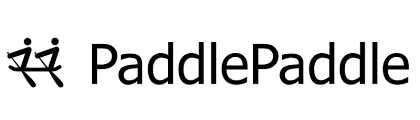
\includegraphics[resolution=100]{PaddlePaddle.png}
		\caption{Logo biblioteki Paddle}
\end{figure}
Pełna nazwa biblioteki PArallel Distributed Deep LEarning. Oprogramowanie skierowane głównie na jeden rynek, mało znane w Europie / USA, jest to zaś najpopularniejszy framework w Chinach. Tworzony i utrzymywany przez firmę Baidu, znany jako Chiński klon Google. Założony w 2000 roku przeniósł pomysł na wyszukiwarkę internetową na chiński rynek i od tej pory z powodzeniem kopiuje wszystkie technologie i pomysły Google, w tym autonomiczne samochody. Jedynym problemem jaki może napotkać osoba nie znająca języka chińskiego jest częste zgłaszanie uwag i komentarzy do kodu bez opisu w języku angielskim. Tutoriale udostępniane w internecie pochodzą głównie od Baidu, stąd bardzo mała popularność poza rodzimym rynkiem. Ze strony domowej można wyczytać często powtarzające się słowa o \"prostocie użycia\", \"prostocie działania\". 

Przechodząc do treści technicznych PaddlePaddle opisywany jest jako zestaw narzędzi i bibliotek do uczenia głębokiego bazujący na \"języku programowania do uczenia głębokich sieci neuronowych\". Biblioteka jest bardzo elastyczna i pozwala na tworzenie dowolnego kształtu modeli. Jak w Tensorflow tak i tutaj istnieje graficzne narzędzie wizualizacji nauczania \"Visual DL\", narzędzie pozwala wyświetlić wydajność trenowania i statystyki danych takie jak dokładność, wartości funkcji kosztu, rozkład parametrów, próbki obrazu i dźwięku, wykres ONNX modelu.

Na podstawie biblioteki istnieje cała społeczność i inicjatywa EasyDL, mająca ułatwić firmom bez specjalistów od algorytmów uczenia maszynowego na wykonanie szybkich i sprawnych modeli bez konieczności posiadania terabajtów danych. Społeczność skupia się głównie w ośrodkach akademickich i startupach w Chinach, gdzie PaddlePaddle jest standardem.

Same możliwości biblioteki są potężne, pozwala na budowę:
\begin{itemize}
\item Botów dzięki technologii Word2Vec,
\item Systemów rekomendacji,
\item Klasyfikatorów obrazów,
\item Translacji maszynowej języków z użyciem głębokiego uczenia,
\item Detekcji obiektów na obrazie filmów z użyciem Single Shot Multibox Detector,
\item Analizatora nastrojów
\end{itemize}

Przy bliższym spotkaniu, widać że jest to klon Tensorflow, który ze względu na brak konkurencji w Chinach jest dużo szybciej rozwijany i jego możliwości w zakresie uczenia na farmach serwerów przewyższają pierwowzór. Z produktów opartych na Baidu korzysta prawie miliard osób, stąd bardzo duży nacisk na optymalizację i własne rozwiązania technologiczne przekładają się na wysoką wydajność.

\noindent
\newline
Dokumentacja: http://paddlepaddle.org/documentation/docs/en/0.15.0/getstarted/index_en.html
\newline
Kod źródłowy: https://github.com/PaddlePaddle/Paddle
\newline
Licencja: Apache 2.0

\subsection{MXNet}
\begin{figure}[h]
	\centering
			
\includegraphics[resolution=100]{MXNet.png}
		\caption{Logo biblioteki MXNet}
\end{figure}
Biblioteka do głębokiego uczenia stworzona przez fundację Apache. Wspiera największą ilość języków ze wszystkich dostępnych bibliotek:
\begin{itemize}
\item Python,
\item C++,
\item Cloujure,
\item Julia,
\item Perl,
\item R,
\item Scala
\end{itemize}
O popularności i powszechne przyjęciu świadczy implementacja na chmurach Microsoft Azure, Intel i Amazon Web Services. Główne zastosowania do których MXNet jest używany to rozpoznawanie mowy i pisma ręcznego, przetwarzanie języka naturalnego i przewidywanie zdarzeń. Użycie skupia się w kręgach przedsiębiorstw, trudno zatem znaleźć badania akademickie przeprowadzane z wykorzystaniem tej biblioteki.

Kolejnym atutem MXNet jest przenośność modeli. Są one zoptymalizowane by nie zajmować dużo pamięci, pozwala to na przeniesienie modelu wytrenowanego w chmurze do urządzenia mobilnego jak smartfon. Łatwe serwowanie modeli, skalowanie na żądanie z mieszaniem GPU i CPU jest zdecydowanie największymi atutami dlaczego Amazon wybrał tą bibliotekę jako pierwszą na swoje centra obliczeniowe. 

Gluon jest API wysokiego poziomu dostarczanym wraz z MXNet. Jego zadaniem jest dostarczyć czystej, spójnej i prostej składni bez obniżania wydajności działania aplikacji. Istnieje również druga warstwa API wysokopoziomowego (można wybierać, z której chce się korzystać) o nazwie Module. Ta warstwa skupia się na pracy z Symbol, paczką do przetwarzania wyrażeń symbolicznych.\cite{DBLP:journals/corr/ChenLLLWWXXZZ15} Jego najlepszymi atutami są:
\begin{itemize}
\item uproszczenie składni budowanych sieci neuronowych, przypominają one pseudokod,
\item elastyczna struktura zapewniająca kod imperatywny,
\item dynamiczny graf sieci, umożliwia zmiany struktury sieci w trakcie działania programu,
\item cache'owanie sieci neuronowej poprawia wydajność, w tym celu używa się modelu sieci HybridSequential
\end{itemize}

\noindent 
\newline
Dokumentacja: https://mxnet.apache.org/api/
\newline
Kod źródłowy: https://github.com/apache/incubator-mxnet
\newline
Licencja: Apache 2.0

\subsection{Caffe2}
\begin{figure}[h]
	\centering
			
\includegraphics[resolution=100, scale=0.35]{Caffe2.png}
		\caption{Logo biblioteki Caffe2}
\end{figure}
Biblioteka wywodzi się z architektury Caffe, narzędzia dla praktyków głębokich sieci neuronowych udostępniającego przejrzystą składnię API w czasach przed pojawieniem się bibliotek wspieranych przez wielkie korporacje. Pierwsza wersja napisana przez Yangqing Jia w trakcie doktoratu na uniwersytecie Berkeley, obecnie jest dyrektorem działu AI w Facebook'u, gdzie rozwijany jest Caffe2. \cite{jia2014caffe} O wieku świadczy dobór języków dostępnych do wykorzystania w bibliotece:
\begin{itemize}
\item C++
\item Python
\item MATLAB
\end{itemize}

Caffe2 jest rozwinięciem tego modelu, również pracuje na GPU, CPU, jest skalowalny, posiada spore wsparcie społeczności. Różnica jest w modyfikacji architektury obliczeniowej. Główną przewagą jest prosta skalowalność na wiele maszyn i urządzenia mobilne. Ta modularność i elastyczność nazywana jest odframeworkowaniem (ang. un-framework) poprzedniej wersji.
\cite{DBLP:journals/corr/JiaSDKLGGD14}

Cała baza została napisana w języku C++ i była testowana latami przez Facebook'a do rozpoznawania obiektów na obrazie, analizy wiadomości do rekomendowania reklam, systemów rekomendujących na podstawie profilu użytkownika. Wydajność jest to jedną z największych zalet, po opracowaniu odpowiedniej architektury, cały kod wdrożeniowy na produkcję może być napisany w C++. Na jednym procesorze NVidia DGX-1 prędkość przetwarznia wynosi 231 obrazów na sekundę.\cite{NvidiaCaffe2(https://developer.nvidia.com/caffe2)}

Caffe2 posiada \"Model ZOO\", gotowe do użycia pretrenowane modele dla najczęściej spotykanych zastosowań bez potrzeby wydawania zasobów na tworzenie modelu od zera. Pełna lista modeli, z którymi można eksperymentować jest pokaźna (na dzień obecny największa ze wszystkich dostępnych \"zwierząt w ZOO\"):
\begin{itemize}
\item AlexNet,
\item GoogleNet,
\item RCNN ILSVRC13,
\item Densenet 121,
\item Detectron,
\item Inception v1,v2,v3,
\item Resnet 50,
\item SqueezeNet,
\item VGG 19,
\item ZFNET 512
\end{itemize}

Dojrzałość produktu sprawiła że istnieje wiele narzędzi programistycznych ułatwiających pracę z biblioteką. Programiści aplikacji mobilnych mają do dyspozycji wtyczki integracyjne do Visual Studio, Android Studio, Xamarin. Dla pozostałych Caffe2 jest dostępne na każdą popularną platformę desktopową oraz w usługach chmurowych. Kod napisany na jedną platforme jest przenoszalny na pozostałe bez konieczności modyfikacji.

Od kwietnia 2018 roku, repozytorium Caffe2 jest przenoszone do katalogu PyTorch. Facebook zdecydował sie na zwiększenie kompatybilności przez stopniowe połączenie bazy kodu. Docelowo Caffe2 ma być modułem dla rozwiązań mobilnych, a PyTorch dla całej reszty.

\noindent
\newline
Dokumentacja: https://caffe2.ai/docs/
\newline
Kod źródłowy: https://github.com/caffe2/caffe2
\newline
Licencja: Apache 2.0 (Caffe 1 -- BSD)


\subsection{ML.NET}
\begin{figure}[h]
	\centering
			
\includegraphics[resolution=100, scale=0.8]{ML_NET.png}
		\caption{Logo biblioteki ML.NET}
\end{figure}
Nowe oprogramowanie od Microsoftu, data wydania pierwszej wersji poglądowej 7 maj 2018. Microsoft tworząc to oprogramowanie wybrał jako grupę docelową programistów skupionych w ekosystemie .NET. API biblioteki udostępnione jest w językach C++ oraz C#, przy czym kompletna dokumentacja jest tylko dla języka C#. Docelowo ma stać się częścią .NET Core. Oprogramowanie od początku istnienia powstaje jako otwartoźródłowe, a Microsoft przy każdym wydaniu zachęca do zgłaszania uwag oraz propozycji dalszego rozwoju lub nowych funkcjonalnośći. Jest to odejście od tradycyjnego modelu utrzymywania oprogramowania w tajemnicy do czasu premiery. Nastawienie na łatwość integracji z oprogramowaniem biznesowym, chmurą Azure oraz łatwość obsługi przez programistów pracujących w technologiach Microsoftu ma zachęcić do wykorzystania oprogramowania na szerszą skalę kiedy wyjdzie ono z fazy rozwojowej i zastąpi CNTK.

W odróżnieniu od pozostałych na chwilę obecną ML.NET jest biblioteką głównie przeznaczną do uczenia maszynowego, wyewulowaną z wewnętrznych rozwiązań Microsoftu od lat używanych w zespołach Windows, Bing, Azure. Microsoft przyznaje że jest to przepisywanie większego systemu do świata otwartego oprogramowania. \cite{https://blogs.msdn.microsoft.com/dotnet/2018/05/07/introducing-ml-net-cross-platform-proven-and-open-source-machine-learning-framework/} Możliwości biblioteki można rozszerzać przez podłączenie modeli z innych bibliotek, wspierane od początku są Tensorflow, Caffe2, CNTK oraz Accord.NET. Sporym atutem jest natywne wsparcie w Azure każdej nowej wersji natychmiast po premierze. Wersja 0.3 przyniosła wsparcie dla formatu modeli ONNX. Narzędzia do głębokiego uczenia pojawiły się w wersji 0.5, zaprezentowanej 12 września 2018. Integracja modeli z Tensorflow umożliwia przeniesienie środowiska z testowego do modelu E2E (ang. Enterprise-2-Enterprise) \"Przedsiębiorstwo-do-przedsiębiorstwa\". Jest to jeszcze zbyt niedojrzała biblioteka by opisywać jej architekturę, nie jest nawet zalecana do rozwiązań produkcyjnych, programiści .NET prawdopodobnie będą z niej chętniej korzystali po pojawieniu się pierwszej kompletnej wersji, co ma nastąpić do wydarzenia BUILD 2019. Obecnie traktowana jest jako sposób na przyciągnięcie do ekosystemu .NET Core osób tworzących rozwiązania dla przedsiębiorstw. ML.NET ma jeszcze wiele braków i wad (konieczność programowania skalowania, brak wsparcia platform mobilnych i wyłączność na chmurę Azure), które uniemożliwiają traktowanie go jako poważnego narzędzia komercyjnego w przeciwieństwie do kolejnego narzędzia Microsoftu CNTK.

\noindent
\newline
Dokumentacja: https://docs.microsoft.com/en-us/dotnet/machine-learning/
\newline
Kod źródłowy: https://github.com/dotnet/machinelearning
\newline
Licencja: MIT

\subsection{CNTK}
\begin{figure}[h]
	\centering
			
\includegraphics[resolution=120]{CNTK.png}
		\caption{Logo biblioteki CNTK}
\end{figure}
Nazwa kompletna \"Microsoft Cognitive Toolkit\". Jest to zestaw narzędzi stworzonych w dziale badań i rozwoju Microsoftu, zajmującego się Deep Learningiem. W 2015 zgodnie z nowym modelem biznesowym, nastawionym na częściowe otwieranie kodu źródłowego narzędzi urzywanych wewnątrz Microsoftu, CNTK został opublikowany na GitHub'ie w kwietniu tego roku. Microsoft wcześniej korzystał z powodzeniem z biblioteki do trenowania modeli usług krytycznych biznesowo. Architektura jest skupiona wokół głębokiego uczenia sieci neuronowych, a dopiero później dodano pozostałe popularne algorytmy uczenia maszynowego.

CNTK posiada zaimplementowane najczęściej używane narzędzia do głębokich sieci neuronowych, takie jak struktury sieci konwolucyjnych czy rekurencyjne sieci neuronowe. Także algorytmy spadku gradientowego i wsteczna propagacja błędów zostały zaimplementowane z automatycznym zrównoleglaniem obliczeń z pojedynczego CPU na wiele procesorów GPU na wielu komputerach w sieci. Biblioteka ta jest jednym z backendów do biblioteki Keras, jednak w przeciwieństwie do Keras'a działa tylko na systemach Windows i wybranych dystrybucjach Linux'a.

Niesamowicie wartościowym atutem jest z pewnością dokumentacja dostarczana przez Microsoft. Nie tylko jest ona przejrzysta i spójna z resztą dokumentacji ekosystemu .NET, ale również dostarcza dziesiątek tutoriali krok po kroku jak budować zaawansowane modele, czyścić dane i wyciągać z nich wnioski. Przestawia nawet w jaki sposób przygotowane już rozwiązania przenieść na chmurę Azure i umożliwić korzystanie z nich klientom. Dla osób nie mających podłoża w Data Science, są gotowe przepisy, czyli przygotowane wcześniej szablony do działania na Azure z interfejsem graficznym instruującym jak przygotować dane aby otrzymać gotową usługę.

\noindent
\newline
Dokumentacja: https://www.microsoft.com/en-us/cognitive-toolkit/
\newline
Kod źródłowy: https://github.com/Microsoft/CNTK
\newline
Licencja: MIT


% ################################
%        ARCHITEKTURA
% ################################

\chapter{Architektura}
\section{Znaczenie architektury dla wydajności sieci}
Elementy sieci neuronowych można ułożyć na nieskończenie wiele sposobów, wystarczy dodać kolejną warstę neuronów lub zmodyfikować wielkość warstwy i wyniki będą zgoła inne. Celem szukania odpowiedniej dla danego zadania architektury jest otrzymanie najlepszej wydajności klasyfikacji przy skończonym i możliwie jak najkrótszym czasie uczenia. Chcąc uzyskać dobre rezultaty bez eksperymentów od zera, należy wybrać architekturę, która została wykorzystana do rozwiązania podobnego zadania bądź przetestować kilka gotowych architektur z wyuczonymi modelami, a następnie sprawdzić jak się zachowują dla posiadanych zbiorów danych na różnych hiperparametrach.

Stworzenie efektywnej architektury przesądziło o wynikach zawodów ''ImageNet Competition 2012''. Pierwsze miejsce w klasyfikacji obrazów wyłącznie z użyciem głębokiej sieci neuronowej zapoczątkowało prawdziwą rewolucję nie tylko wśród społeczności uczenia maszynowego, ale całego przemysłu technologicznego. Pierwszy zespół, któremu udało się zejść z błędem rozpoznania do mniej niż 25\% Geuffrey Hinton, zwany ojcem chrzestnym głębokich sieci neuronowych (ang. Godfather of Deep Learning) udowodnił że jego przekonania, którymi się kierował w trakcie kilkudziesięcioletniej kariery naukowej są słuszne. Poprzeczką, której profesor Hinton nie mógł wcześniej przeskoczyć były ograniczenia obliczeniowe procesorów, kiedy technologia GPU wraz z możliwością programowania równoległego w CUDA umożliwiły przetestowanie idei, podejście do rozpoznawania obrazów zmieniło świat przemysłu, a wkrótce zmieni życie każdego człowieka.

Rok 2017 został uznany za czas kiedy ImageNet Competition został na stałe rozwiązany. Błędne rozpoznanie algorytmów wśród najlepszych drużyn wyniosło zaledwie 2\%. Przez pięć lat od czasu debiutu AlexNet powstało wiele architektur sieci neuronowych, bibliotek wyspecjalizowanych w szybkim tworzeniu nowych prototypów, a te dające obiecujące wyniki zostały podzielone względem zastosowania. Obecnie wyróżniane typy sieci neuronowych są sklasyfikowane wzgledem typu danych wejściowych. Dla sygnału wejściowego w postaci pikseli najlepiej sprawdza się konwolucyjna sieć neuronowa. Warstwy konwolucyjne potrafią bardzo dokładnie wyodrębnić cechy obrazu na różnych poziomach złożoności co jest wyjaśnione w dalszej części pracy.

Polskim ekspertem i popularyzatorem sieci neuronowych od wielu lat jest profesor doktor habilitowany inżynier Ryszard Tadeusiewicz. Osoba bardzo zasłużona w naukach technicznych. Jego książki stały się częścią bibliografi niniejszej pracy. Profesor w swoich publikacjach istotnie zwraca uwagę na architekturę jako element konieczny w budowaniu 

Architektury różnią się ilością warstw ukrytych, typem neuronów i funkcji aktywacji w każdej warstwie. 
“Właśnie taka [warstwowa] struktura sieci wyjątkowo łatwo i wygodnie da się wytwarzać zarówno w formie modelu elektronicznego, jak i da się symulować w formie programu komputerowego. Dlatego badacze przyjęli właśnie strukturę warstwową i od tej pory stosują ją we wszystkich sztucznych sieciach neuronowych. [...] W związku z tym wszyscy tak postępują, nie martwiąc się ani przesłankami biologicznymi, ani dowodami wskazującymi, że architektura sieci bardziej wymyślnie dostosowanej do charakteru zadania może znacznie lepiej realizować stawiane zadania.”

Tak napisał w 2007 roku, kiedy nie istniały jeszcze złożone głębokie sieci neuronowe, największe w tej porzy miały 5 warstw ukrytych, a zbiory danych na których pracowano były stosunkowo niewielkie w porównaniu z dzisiejszymi zasobami skatalogowanych obrazów. Prof. Tadeusiewicz uważa że jest to najlepsze ułożenie neuronów ze względu na prostotę oraz dowód że badacze znaleźli podobne struktury w niektórych częściach ludzkiego mózgu (w tym w oku, które jest ewolucyjnie złożone z tej sameh tkanki co mózgowa).

Dowodem na znaczenie ułożenia neuronów w poprawnej strukturze jest ich rosnąca skuteczność od kiedy badacze bardzo dużo eksperymentują z różnymi kombinacjami. Coroczne zawody ImageNet, w których udowadnia się że struktura sieci ma znaczenie są świetnym przykładem że jest to proces iteracyjny i jak podkreślano wcześniej, metoda empiryczna jest obecnie jedynym sposobem na znalezienie idealnego modelu.

\section{Przegląd najbardziej efektywnych architektur}

\subsection{LeNet}
[Yann LeCun, Leon Bottou, Yoshua Bengio, Patrick Haffner, 1998] - . Pierwsze praktyczne zastosowanie sieci konwolucyjnych jeszcze w latach 90’tych. Używana była do prostych zadań: czytanie kodów pocztowych, liczb.\cite{Lecun98gradient-basedlearning}

\begin{figure}[h]
	\centering
			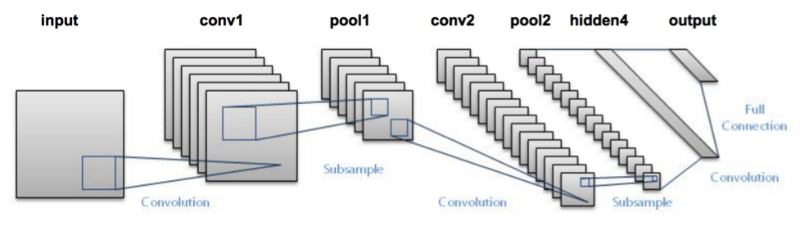
\includegraphics[resolution=100, scale=0.6]{LeNet.png}
		\caption{Architektura sieci LeNet}
\end{figure}

\subsection{AlexNet}
 [Alex Krizhevsky, Ilya Sutskever, Geoffrey E. Hinton, 2012] - pierwsza prawdziwa konwolucyjna sieć neuronowa (CNN), która pomogła zmienić opinię na temat uczenia głębokiego. Została zaimplementowana z użyciem biblioteki CUDA. Pierwsza sieć neuronowa, ucząca się z powodzeniem dla dużego zbioru danych.
 Została wytrenowana na zbiorze danych złożonym z ponad 15 milionów obrazów podzielonych na 22000 klas. 
 W testach top-1 i top-5 uzyskała wartości kolejno 37,5\% i 17\%, co pozwoliło wygrać konkurs ImageNet Large Scale Visual Recognition Challenge. 
 Sieć neuronowa zawiera 60 milionów parametrów i 650 000 neuronów. Architekturę tworzy 8 warstw, gdzie pierwsze 5 to warstwy konwolucyjne, a pozostałe 3 są warstwami w pełni połączonymi, ta ostatnia ma oczywiście 1000 wyjść z funkcji softmax. AlexNet znacząco przewyższyła swoją wydajnością poprzednich uczestników i wygrała zawody redukując błąd top-5 do 15,32\%. Drugie miejsce to błąd ok 26.2\% (nie była to CNN). Sieć jest głęboką modyfikacją architektury Yann’a LeCunn’a. AlexNet była zaplanowana na dwie karty graficzne, stąd rozdzielenie przepływu informacji na 2 części. Trenowanie sieci na 2 GPU było nowością na te czasy. Sieć została wytrenowana na zbiorze ImageNet. Do wyliczenia funkcji nieliniowych były używane ReLU (tutaj po raz pierwszy okazało się że ReLU działa dużo szybciej niż tangens hiperboliczny). Sieć o której będą uczyły się dzieci na lekcjach historii. \cite{NIPS2012_4824}

\begin{figure}[h]
	\centering
			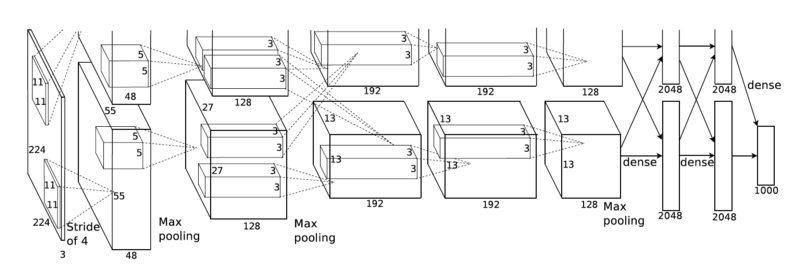
\includegraphics[resolution=100, scale=0.7]{AlexNet.png}
		\caption{Architektura sieci AlexNet}
\end{figure}



\subsection{VGG Net}
 [Simoyan i Zisserman, 2014] - sieć złożona z 16 warstw konwolucyjnych, która charakteryzuje się małymi filtrami i duża głębokość sieci.
W trakcie trenowania sieci wyjście jest ustawione na ustalony rozmiar (224 x 224 x 3). Przetwarzanie wstępne obejmuje odjęcie mediany wartości RGB dla każdego piksela. Zdjęcie jest przetwarzanie przez stos warstw konwolucyjnych, gdzie używane są filtry o bardzo małym polu widzenia (3x3) [najmniejszy możliwy rozmiar by móc rozpoznać kierunek]. Operacja Max-pooling jest wykonana na polu 4 pikseli, co pokazuje że jest to pobieranie jak najmniejszych cech z obrazu. Ukryte warstwy są wyposażone w nieliniową funkcję aktywacji ReLU. Po stosie warstw konwolucyjnych, następuje nałożenie 3 warstw w pełni połączonych (to takie duże warstwy zawierające wszystkie cechy?). Pierwsze dwie mają 4096 kanałów, trzecia już tylko 1000 (po jednym kanale na klasę obiektu). Obecnie architektura ta jest dość popularnym wyborem dla wyodrębniania cech ze zdjęć. Konfiguracje wag dla zbioru obrazów z ImageNet są dostępne online. W tej sieci problemem jest 140 milionów parametrów, którymi czasem trzeba zarządzać. \cite{DBLP:journals/corr/SimonyanZ14a}

\subsection{GoogleNet / Inception}
[Christian Szegedy, Wei Liu, Yangqing Jia, Pierre Sermanet, Scott Reed, Dragomir Anguelov, Dumitru Erhan, Vincent Vanhoucke, Andrew Rabinovich, 2014] - produkt jak nazwa wskazuje wyszedł z firmy Google. Charakteryzuje się przełomową poprawą użycia zasobów wewnętrznych. ImageNet jest zaprojektowana na jak największą szerokość i głębokość jednocześnie utrzymując stałe zużycie mocy obliczeniowej. Optymalizacja jakości opiera się na zasadzie Hebbian’a (jest to teoria neuronauki, która mówi o adaptacji neuronów w trakcie nauki). Błędy klasyfikacji wynoszą top-1: 17,2\% i top-5: 3,58\% (dla v3). Sieć składa się łącznie z 22 warstw. Sieć jest modułowa, gdzie każdy moduł pełni rolę wielopoziomowego ekstraktora cech przeliczającego konwolucje na macierzach rozmiarów 1x1, 3x3, 5x5. Zaletą tej architektury są bardzo małe rozmiary wag (mniej niż 100MB dla v3). Kolejną ważną zaletą jest ilość parametrów, tylko 4 miliony co jest wynikiem 12 razy lepszym od AlexNet. Jest to jedna z najbardziej złożonych sieci względem architektury modułowej. W wersji naiwnej każda warstwa posiada 4 ekstraktory cech (3 konwolucyjne i jedną 3x3 max pooling), następnie wartości te są składane i wysyłane do warstwy wyżej. Do poprawienia wydajności obliczeniowej pozbyto się warstwy “w pełni połączonej”. \cite{DBLP:journals/corr/SzegedyLJSRAEVR14}

\subsection{ResNet}
[Kaiming He et al, 2015]  - architektura oparta na mikro modułach. Charakteryzuje się możliwością odrzucania połączeń i posiada ogromny moduł na normalizację zbioru iteracji (batch normalization). Normalizacja jest pomysłem zaczerpniętym z rekurencyjnych sieci neuronowych. Ta technika pozwala stworzyć sieć ze 152 warstwami ukrytymi przy zachowaniu złożoności mniejszej niż VGG. \cite{DBLP:journals/corr/XieGDTH16}
\begin{figure}[h]
	\centering
			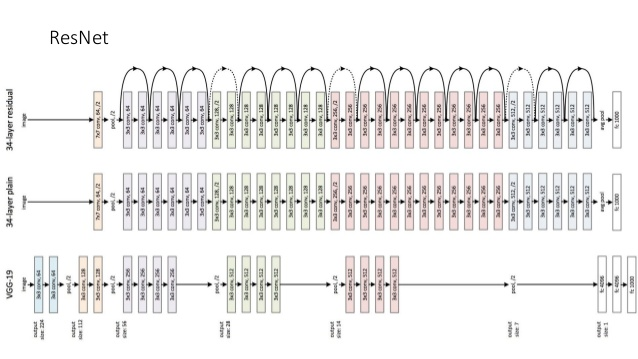
\includegraphics[resolution=100]{ResNet.png}
		\caption{Architektura sieci ResNet}
\end{figure}

\subsection{ResNeXt}
[Saining Xie, Ross Girshick, Piotr Dollar Zhuowen Tu Kaiming He, 2017] - modularyzowalna 
\cite{DBLP:journals/corr/XieGDTH16}
\begin{figure}[h]
	\centering
			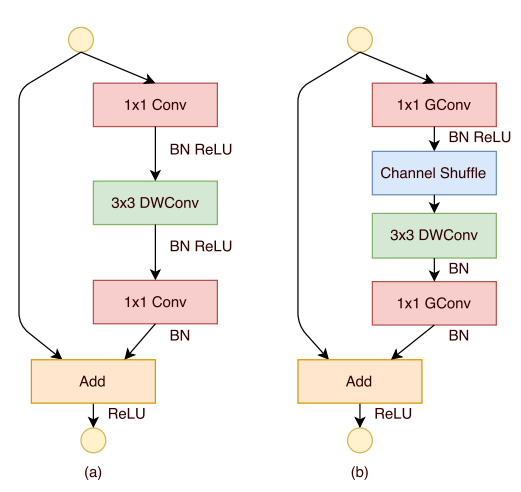
\includegraphics[resolution=120]{ResNeXt.png}
		\caption{Architektura sieci ResNeXt}
\end{figure}

\subsection{RCNN -- obrazek jest zastępczy nie ma nic w internecie interesującego (zrobić własną wizualizację)}
[Authors, Year] - \cite{DBLP:journals/corr/RenHG015}
\begin{figure}[h]
	\centering
			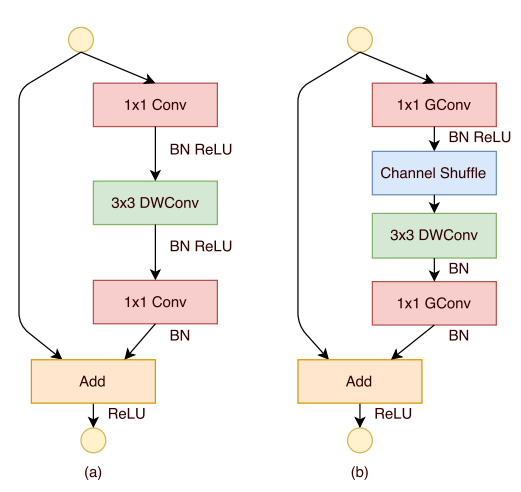
\includegraphics[resolution=120]{ResNeXt.png}
		\caption{Architektura sieci RCNN}
\end{figure}

\subsection{YOLO - You Only Look Once}
[Joseph Redmon, Santosh Divvala, Ross Girshick, Ali Farhadi, 2016] - You Only Look Once jest systemem wykrywania obiektów w czasie rzeczywistym. Obraz jest dzielony na części oddzielonymi od siebie prostokątami.
Cały przepływ danych do wykrycia obiektów jest jedną siecią, dlatego może być zoptymalizowany \cite{DBLP:journals/corr/RedmonDGF15}
\begin{figure}[h]
	\centering
			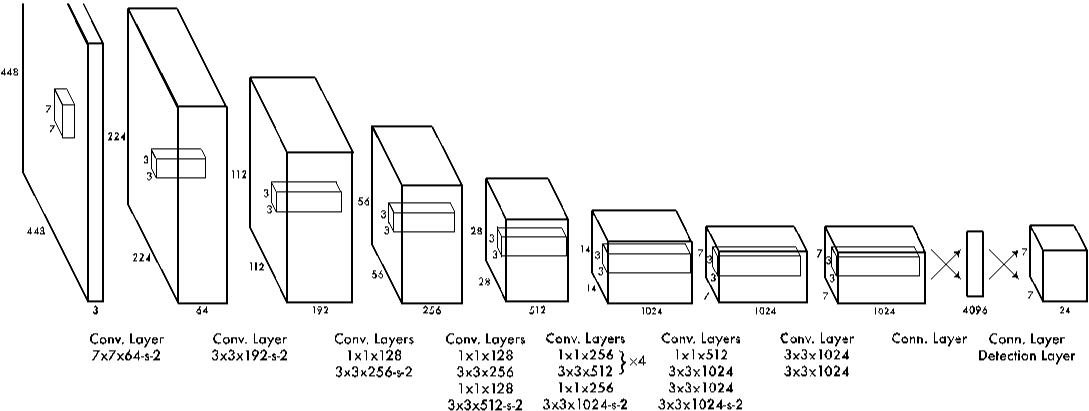
\includegraphics[resolution=100, scale=0.6]{YOLO.png}
		\caption{Architektura sieci YOLO}
\end{figure}

\subsection{SqueezeNet}
[Authors, Year] - \cite{DBLP:journals/corr/IandolaMAHDK16}
\begin{figure}[h]
	\centering
			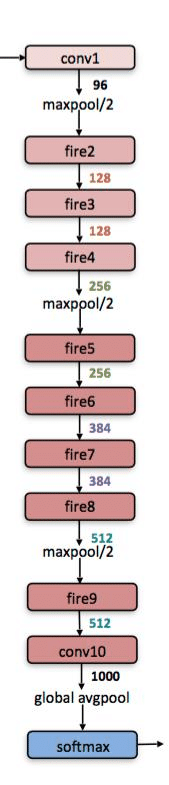
\includegraphics[resolution=100, scale=0.8]{SqueezeNet.png}
		\caption{Architektura sieci SqueezeNet}
\end{figure}

\subsection{SegNet}
[Authors, Year] - \cite{DBLP:journals/corr/BadrinarayananH15}
\begin{figure}[h]
	\centering
			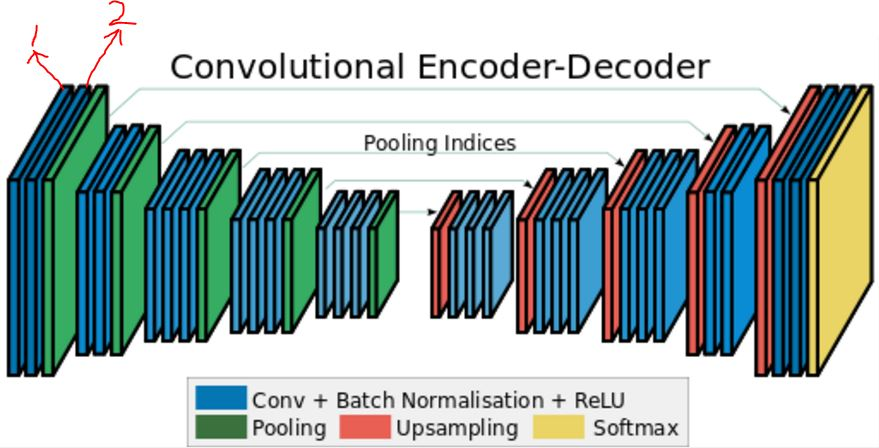
\includegraphics[resolution=100, scale=0.5]{SegNet.png}
		\caption{Architektura sieci SegNet}
\end{figure}

\subsection{Generative Adversarial Network}
[Ian J. Goodfellow, Jean Pouget-Abadie, Mehdi Mirza, Bing Xu, David Warde-Farley, Sherjil Ozair†, Aaron Courville, Yoshua Bengio‡, 2014] - w skrócie GAN. Są architekturą sieci neuronowych skomponowanych z dwóch sieci przeciwstawionych wobec siebie. Zaprojektowane na uniwersytecie w Montrealu (gdzie powstało większość przełomów dotyczących neuronów) przez największe obecnie autorytety w dziedzinie. GAN obudził duże nadzieje na szybkie i "twórcze" działania algorytmów, jego najczęstszym zastosowaniem jest tworzenie komputerowych "dzieł sztuki". Jak to działa? Jedna sieć generuje kandydatów, a druga ich ocenia wytworzone obiekty. W ten sposób obie sieci uczą się od siebie wzajemnie. - \cite{NIPS2014_5423}
\begin{figure}[h]
	\centering
			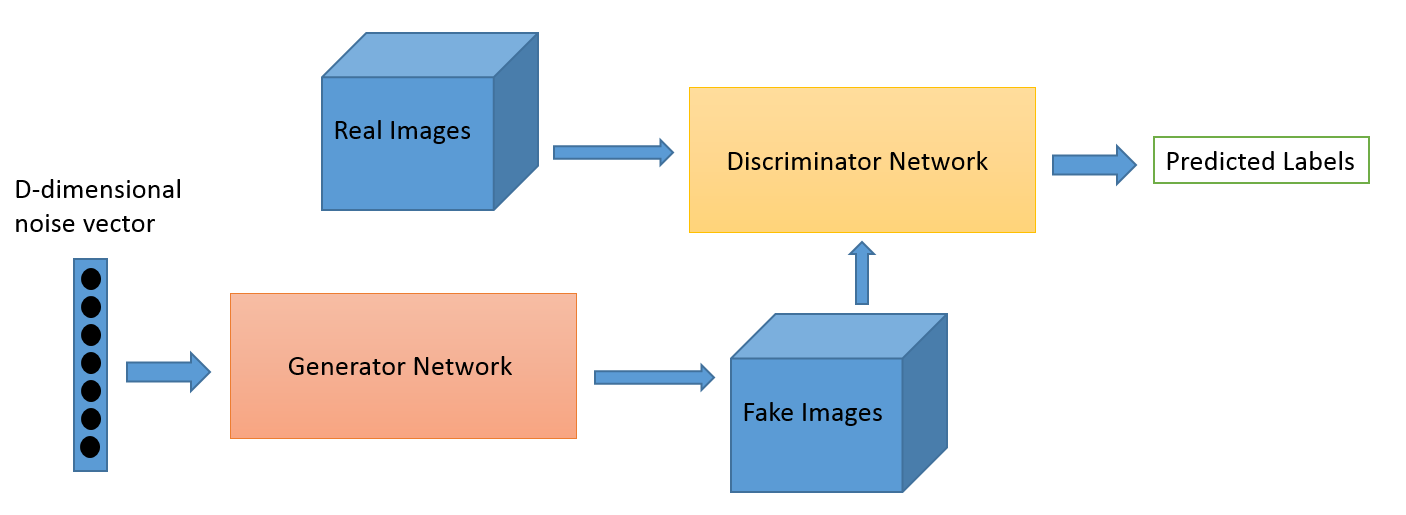
\includegraphics[resolution=100,scale=0.3]{GAN.png}
		\caption{Architektura sieci GAN}
\end{figure}


% ################################
%        PORÓWNANIE WYDAJNOŚCI ARCHITEKTUR
% ################################
\chapter{Testy wydajności}

% ################################
%        PODSUMOWANIE
% ################################

\chapter*{Podsumowanie}
\markboth{}{Podsumowanie}
\addcontentsline{toc}{chapter}{Podsumowanie}

% ################################
%        SPIS RYSUNKÓW
% ################################

\addcontentsline{toc}{chapter}{Spis rysunków}
\listoffigures

% ################################
%        BIBLIOGRAFIA
% ################################
\bibliographystyle{plain}
\bibliography{bibliography/alexnetNips,bibliography/deeplearningbook,bibliography/dropout,bibliography/fastAI,bibliography/ganArxiv,bibliography/googleNet,bibliography/lecun,bibliography/medicalImage,bibliography/microsoftResNet,bibliography/rCNN,bibliography/relu,bibliography/resnextArxiv,bibliography/VGGNet,bibliography/ZFNet,bibliography/YOLO,bibliography/SqueezeNet,bibliography/SegNet,bibliography/deeplearningAI,bibliography/deeplearningTensorflow,bibliography/odkrywanieSieci,bibliography/benchmarks,bibliography/MXNet,bibliography/CaffePerformance,bibliography/caffe} 

\end{document}